%%%%%%%%%%%%%%%%%%%%%%%%%%%%%%%%%%%%%%%%%
% Short Sectioned Assignment LaTeX Template Version 1.0 (5/5/12)
% This template has been downloaded from: http://www.LaTeXTemplates.com
% Original author:  Frits Wenneker (http://www.howtotex.com)
% License: CC BY-NC-SA 3.0 (http://creativecommons.org/licenses/by-nc-sa/3.0/)
%%%%%%%%%%%%%%%%%%%%%%%%%%%%%%%%%%%%%%%%%

%----------------------------------------------------------------------------------------
%	PACKAGES AND OTHER DOCUMENT CONFIGURATIONS
%----------------------------------------------------------------------------------------

\documentclass[paper=a4, fontsize=11pt]{scrartcl} % A4 paper and 11pt font size

% ---- Entrada y salida de texto -----

\usepackage[T1]{fontenc} % Use 8-bit encoding that has 256 glyphs
\usepackage[utf8]{inputenc}
%\usepackage{fourier} % Use the Adobe Utopia font for the document - comment this line to return to the LaTeX default

% ---- Idioma --------

\usepackage[spanish, es-tabla]{babel} % Selecciona el español para palabras introducidas automáticamente, p.ej. "septiembre" en la fecha y especifica que se use la palabra Tabla en vez de Cuadro

% ---- Otros paquetes ----

\usepackage{url} % ,href} %para incluir URLs e hipervínculos dentro del texto (aunque hay que instalar href)
\usepackage{amsmath,amsfonts,amsthm} % Math packages
%\usepackage{graphics,graphicx, floatrow} %para incluir imágenes y notas en las imágenes
\usepackage{graphics,graphicx, float} %para incluir imágenes y colocarlas

% Para hacer tablas comlejas
%\usepackage{multirow}
%\usepackage{threeparttable}

%\usepackage{sectsty} % Allows customizing section commands
%\allsectionsfont{\centering \normalfont\scshape} % Make all sections centered, the default font and small caps

\usepackage{fancyhdr} % Custom headers and footers
\pagestyle{fancyplain} % Makes all pages in the document conform to the custom headers and footers
\fancyhead{} % No page header - if you want one, create it in the same way as the footers below
\fancyfoot[L]{} % Empty left footer
\fancyfoot[C]{} % Empty center footer
\fancyfoot[R]{\thepage} % Page numbering for right footer
\renewcommand{\headrulewidth}{0pt} % Remove header underlines
\renewcommand{\footrulewidth}{0pt} % Remove footer underlines
\setlength{\headheight}{13.6pt} % Customize the height of the header

\numberwithin{equation}{section} % Number equations within sections (i.e. 1.1, 1.2, 2.1, 2.2 instead of 1, 2, 3, 4)
\numberwithin{figure}{section} % Number figures within sections (i.e. 1.1, 1.2, 2.1, 2.2 instead of 1, 2, 3, 4)
\numberwithin{table}{section} % Number tables within sections (i.e. 1.1, 1.2, 2.1, 2.2 instead of 1, 2, 3, 4)

\setlength\parindent{0pt} % Removes all indentation from paragraphs - comment this line for an assignment with lots of text

\newcommand{\horrule}[1]{\rule{\linewidth}{#1}} % Create horizontal rule command with 1 argument of height

\graphicspath{ {./images/} }

%----------------------------------------------------------------------------------------
%	TÍTULO Y DATOS DEL ALUMNO
%----------------------------------------------------------------------------------------

\title{	
	\normalfont \normalsize 
	\textsc{\textbf{Inteligencia de Negocio (2018-2019)} \\ Doble Grado en Ingeniería Informática y Matemáticas \\ Universidad de Granada} \\ [25pt] % Your university, school and/or department name(s)
	\horrule{0.5pt} \\[0.4cm] % Thin top horizontal rule
	\huge Memoria Práctica 2: \\ Segmentación para Análisis Empresarial. Grupo de Prácticas 1 \\ % The assignment title
	\horrule{2pt} \\[0.5cm] % Thick bottom horizontal rule
}

\author{Luis Balderas Ruiz \\ \texttt{luisbalderas@correo.ugr.es}} 
% Nombre y apellidos 

\date{\normalsize\today} % Incluye la fecha actual

%----------------------------------------------------------------------------------------
% DOCUMENTO
%----------------------------------------------------------------------------------------

\begin{document}
	
\maketitle % Muestra el Título
	
\newpage %inserta un salto de página
	
\tableofcontents % para generar el índice de contenidos
	
\listoffigures
	
\listoftables
	
\newpage



%----------------------------------------------------------------------------------------
%	Introducción
%----------------------------------------------------------------------------------------

\section{Introducción}

La Estadística tiene cada vez más influencia en la sociedad. En los periódicos aparecen diariamente resultados estadísticos sobre economía, salud, opinión o política. ¿Qué hay de cierto en la estadística? Podemos desvirtuar la verdad con estadísticas, pero podemos especular más sin ellas. La Estadística es necesaria cuando los fenómenos objeto de estudio no se pueden predecir con exactitud, por tener una componente de azar, de incertidumbre. Dicho azar ya no es el producto de nuestro ignorancia, sino una expresión de nuestro conocimiento. La incertidumbre se puede controlar y cuantificar gracias a la estadística.

Cuando las estadísticas están basadas en datos ciertos podemos proporcionar una información muy valiosa a la sociedad. En ese sentido, el Instituto Nacional de Estadística (INE) es el ente público dedicado a la elaboración de recoger datos de la población para así plasmar numéricamente la realidad que vivimos. Concretamente, en 2011 se publicó el censo de población (\cite{censo}), que será nuestro objetivo de estudio. El conjunto de datos se compone de 142 variables sobre sexo, edad, nacionalidad, estudios... Nos centraremos en los datos relativos a la provincia de Granada, lo que se reduce a 83499 casos. 

El presente estudio estadístico se centra en cuatro casos:
\begin{itemize}
	\item Caso 1: Personas que viven con sus padres. 
	\item Caso 2: Mujeres científicas.
	\item Caso 3: Hogares biparentales con hijos menores de 25 años.
	\item Caso 4: Mujeres y hogar.
\end{itemize}

Dichos casos se enfrentarán mediante técnicas de clustering. Más concretamente, a través de 4 algoritmos basados en particionamiento, como son kMeans (\cite{kmeans}), MeanShift (\cite{ms}), BIRCH (\cite{birch}, \cite{zhang1996birch}) y DBSCAN (\cite{dbscan}); y uno jerárquico aglomerativo tipo Ward (\cite{ward}). Su análisis se apoya en datos de rendimiento como gráficos tipo \textit{scatter matrix, heatmap o dendograma}, según el algoritmo. Además, los algoritmos basados en particionamiento se evaluarán a través de las métricas \textit{Silhouette} y \textit{Calinski-Harabaz}. \\

Por último, es necesario reseñar que por propia definición, algunos algoritmos requieren la especificación del número de clusters a formar, mientras que otros, dados ciertos parámetros, muestran el número de cluster óptimo asociado a dicha configuración. He probado distintas configuraciones de cada algoritmo (se especificarán en cada apartado), pero en el caso de kMeans utilizo el llamado \textit{Elbow Method} para elegir el número óptimo de clusters (\cite{elbow-method}, \cite{elbow-method1}).

\newpage
%----------------------------------------------------------------------------------------
%	Caso de estudio X 
%----------------------------------------------------------------------------------------


\section{Caso de estudio 1: Personas que viven con sus padres}

El presente caso de estudio se basa en la búsqueda de patrones entorno a personas que viven con sus padres. Para extraer dicho subconjunto de instancias, se filtra por \textit{EDADMAD>0} y \textit{EDADPAD>0}. Además, he elegido las siguientes características:
\begin{itemize}
	\item EDAD
	\item ESREAL
	\item CMUNN
	\item ESTUMAD
	\item ESTUPAD
\end{itemize}

\begin{figure}[H] %con el [H] le obligamos a situar aquí la figura
	\centering
	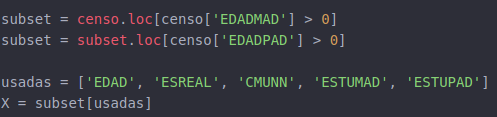
\includegraphics[scale=0.5]{c1-1.png}  %el parámetro scale permite agrandar o achicar la imagen. En el nombre de archivo puede especificar directorios
	\caption{Configuración del caso 1} 
	\label{fig:configuración-caso1}
\end{figure}

con la pretensión de encontrar relaciones entre la edad, los estudios del sujeto, el lugar donde vive y la formación de sus progenitores. Los resultados son los siguientes:

\subsection{kMeans}

\begin{figure}[H] %con el [H] le obligamos a situar aquí la figura
	\centering
	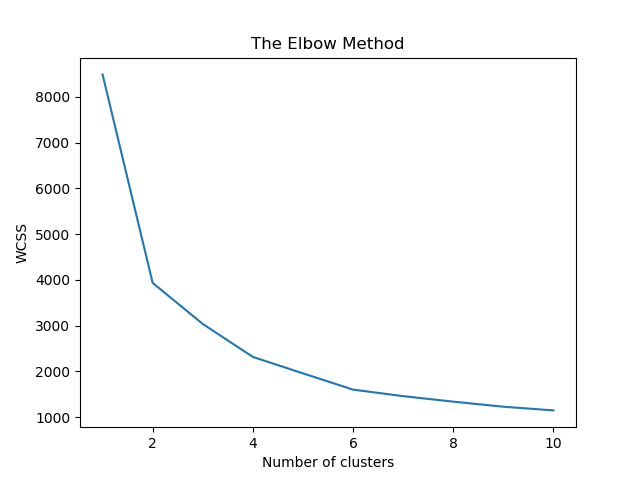
\includegraphics[scale=0.6]{em1.png}  %el parámetro scale permite agrandar o achicar la imagen. En el nombre de archivo puede especificar directorios
	\caption{Salida de Elbow Methow} 
	\label{fig:em-caso1}
\end{figure}

Elbow Method nos indica que el número óptimo de clusters es 2. En efecto, así es tras varias configuraciones distintas:

\begin{table}[H]
	\begin{tabular}{|c|c|c|c|c|}
		\hline
		Nº Clusters & Tiempo(s) & Silhoutte & Calinski-Harabaz & Tamaño de cada cluster                                                                                                    \\ \hline
		2           & 0.08      & 0.51388   & 24903.026        & \begin{tabular}[c]{@{}c@{}}1: 11690 (54.34\%)\\ 0: 9824 (45.66\%)\end{tabular}                                            \\ \hline
		3           & 0.15      & 0.44672   & 19309.672        & \begin{tabular}[c]{@{}c@{}}1:  9824 (45.66\%)\\ 2:  5988 (27.83\%)\\ 0:  5702 (26.50\%)\end{tabular}                      \\ \hline
		4           & 0.29      & 0.40962   & 19109.260        & \begin{tabular}[c]{@{}c@{}}2:  5988 (27.83\%)\\ 1:  5702 (26.50\%)\\ 3:  5180 (24.08\%)\\ 0:  4644 (21.59\%)\end{tabular} \\ \hline
	\end{tabular}
\end{table}

A la luz de Silhoutte y Calinski-Harabaz, la configuración con dos clusters es la más conveniente. A continuación muestro las representaciones gráficas:

\begin{figure}[H] %con el [H] le obligamos a situar aquí la figura
	\centering
	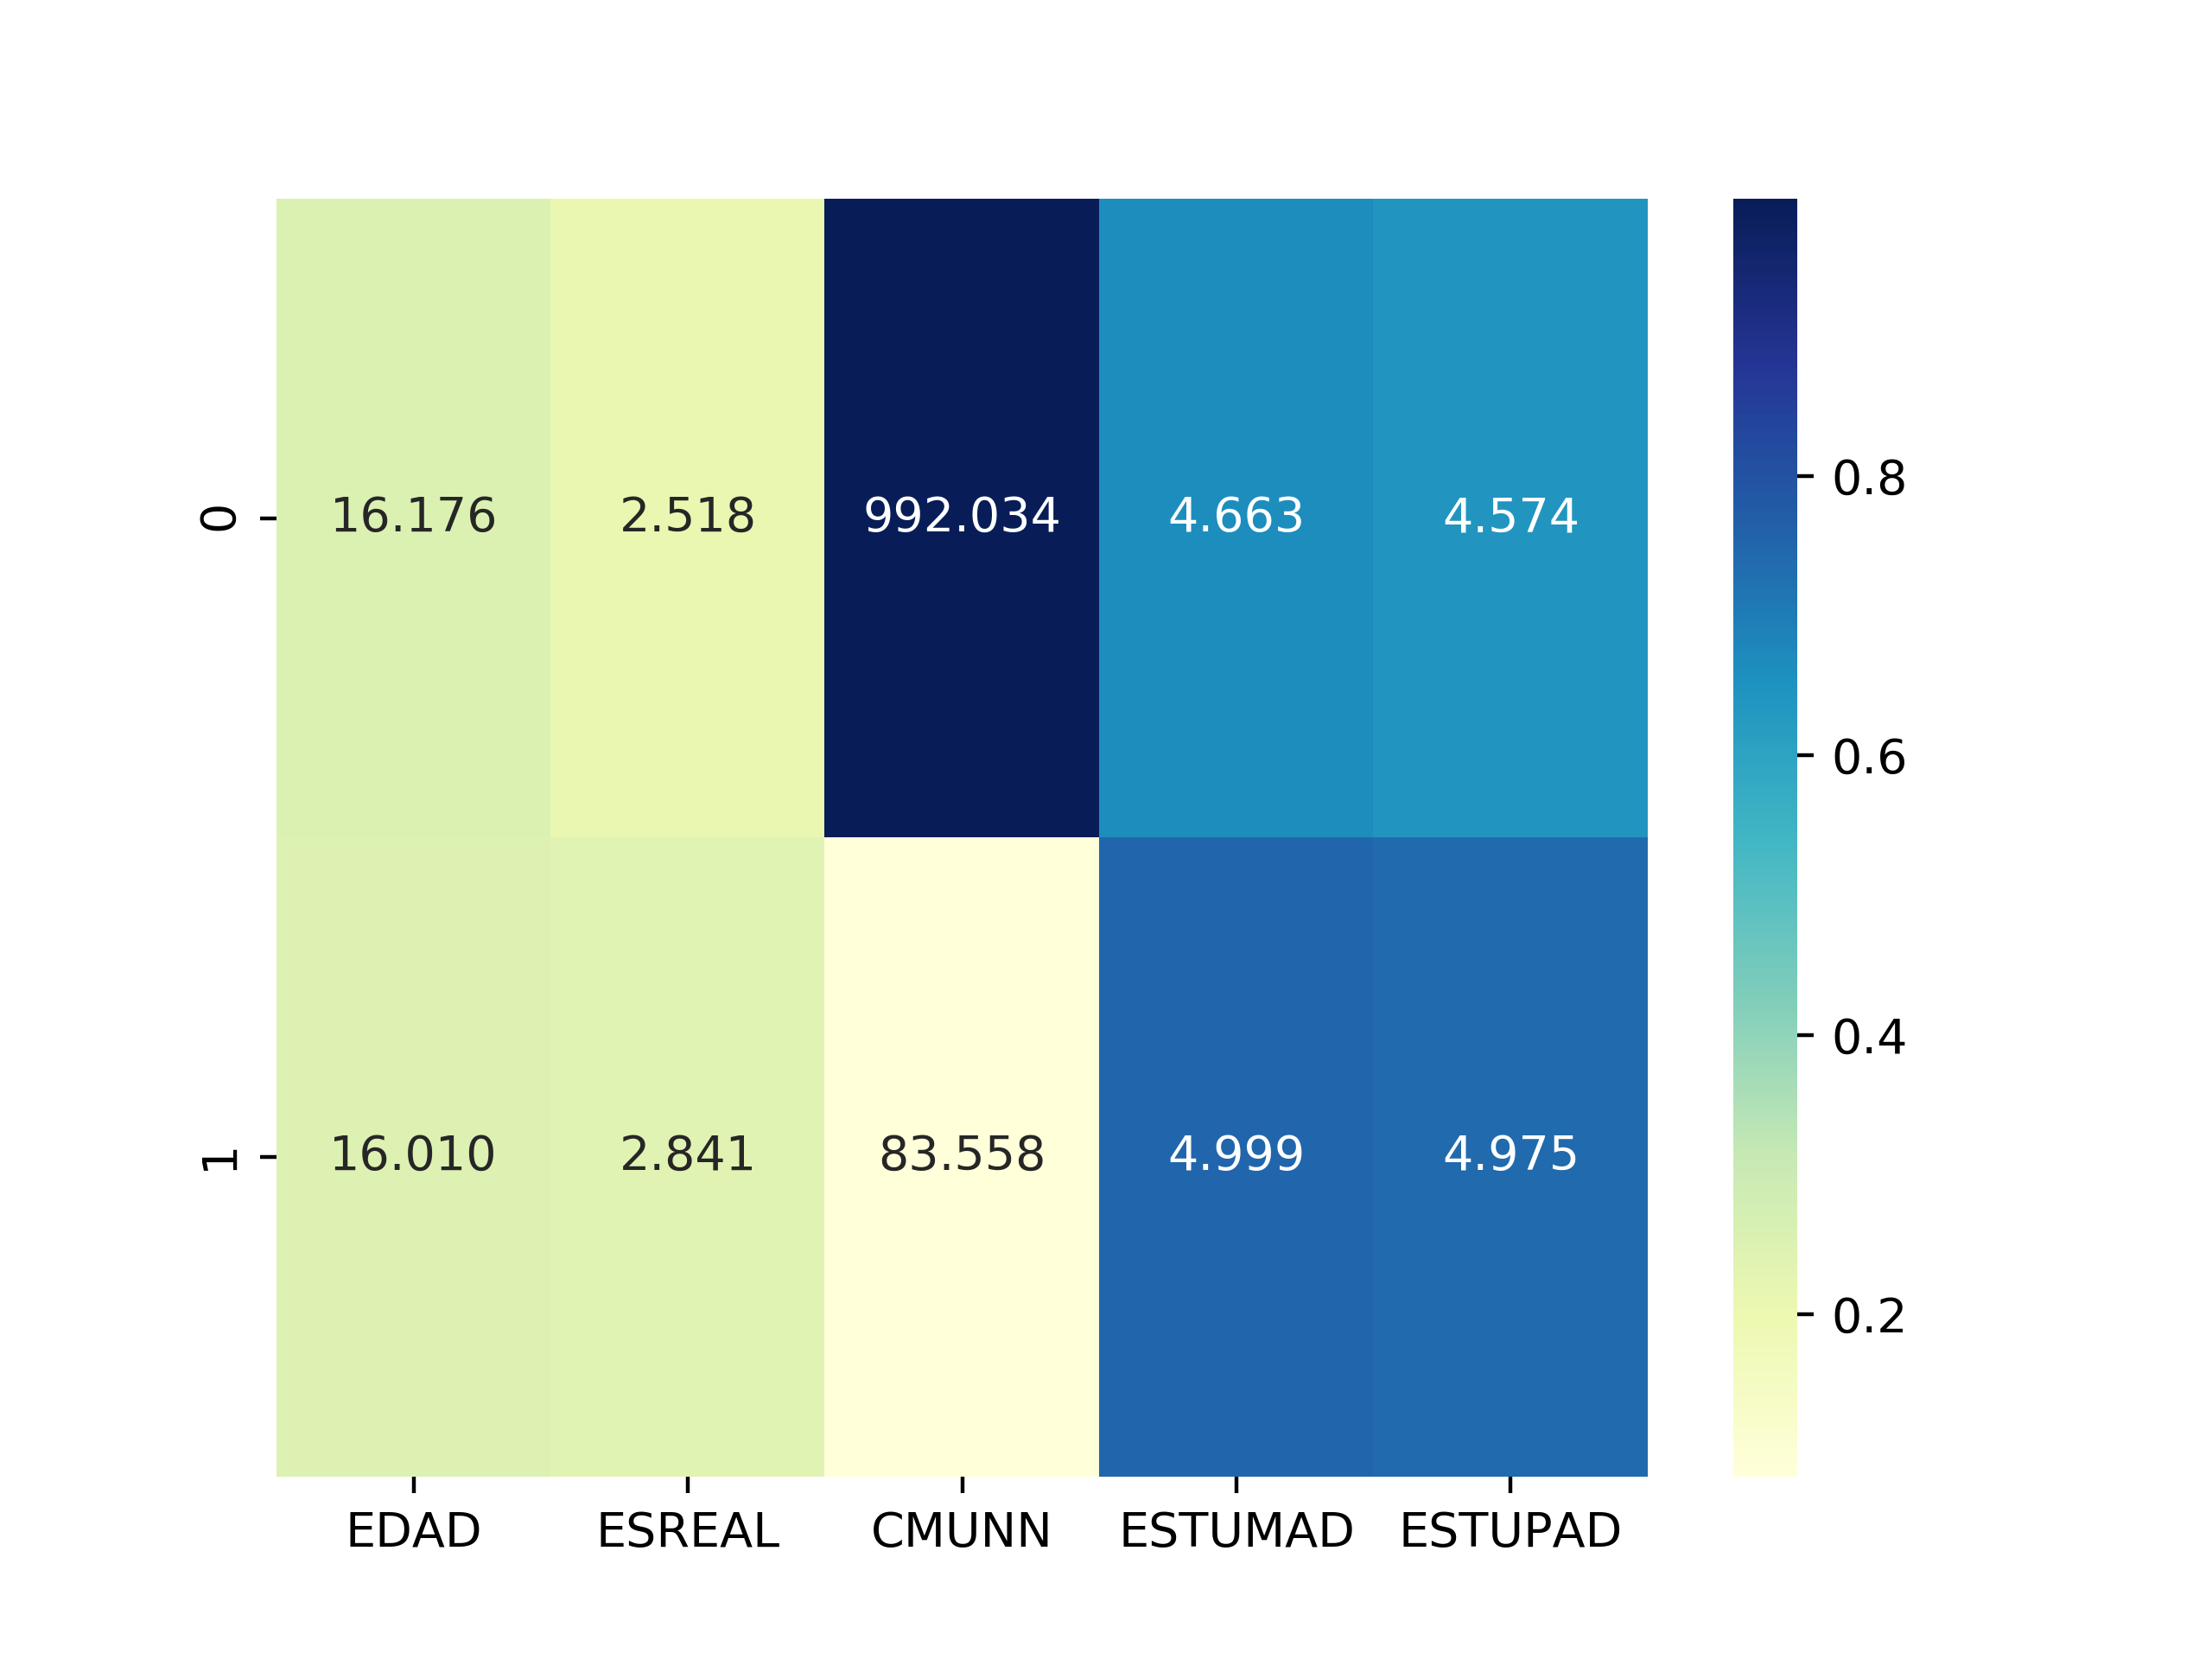
\includegraphics[scale=0.8]{heatmap-km-1.png}  %el parámetro scale permite agrandar o achicar la imagen. En el nombre de archivo puede especificar directorios
	\caption{Heatmap kMeans Caso 1} 
	\label{fig:hm-km-caso1}
\end{figure}

\begin{figure}[H] %con el [H] le obligamos a situar aquí la figura
	\centering
	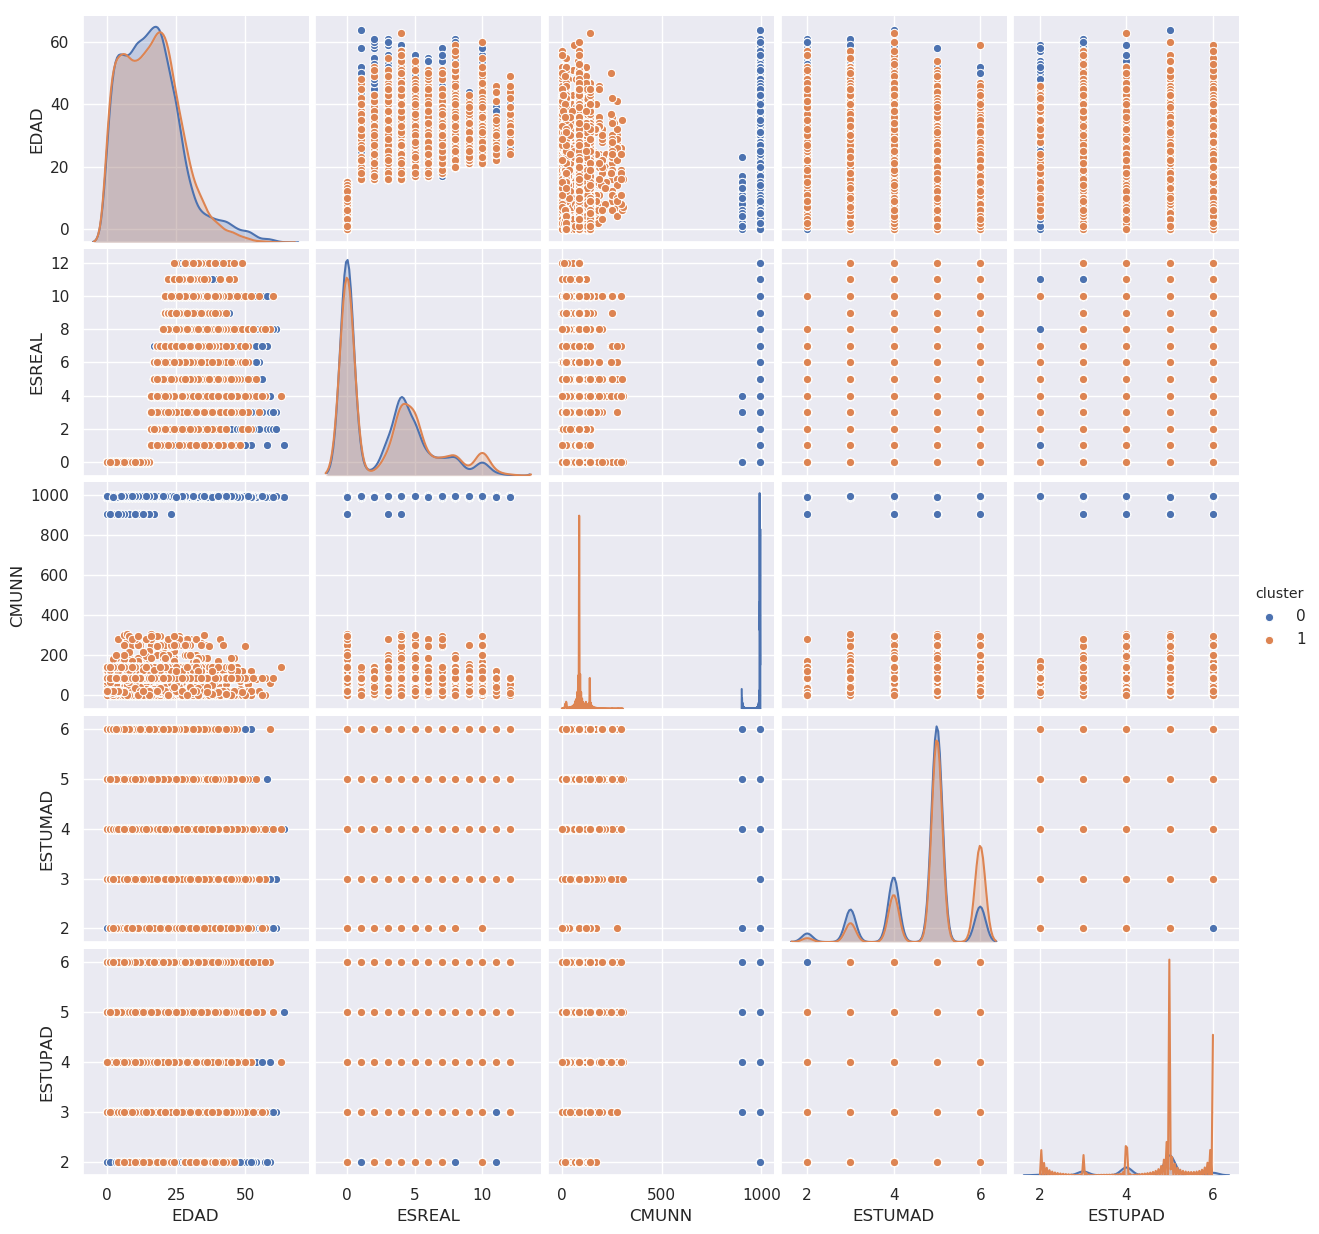
\includegraphics[scale=0.4]{kmeans-1.png}  %el parámetro scale permite agrandar o achicar la imagen. En el nombre de archivo puede especificar directorios
	\caption{Scatter kMeans Caso 1} 
	\label{fig:sc-km-caso1}
\end{figure}

Como se puede comprobar tanto en el heatmap como con el scatter matrix (con mayor profundidad), cuatro de las cinco características elegidas (edad,estudios y formación de los padres) son bastante parecidas. Lo que hace diferenciar claramente a los dos grupos de individuos es el código o tamaño del municipio donde residen, encontrándose un grupo de individuos que nacieron en un municipio de entre 2000 y 5000 habitantes, mientras que el otro grupo tiene una población de más de 20000 habitantes. Por lo general, los sujetos suelen tener 16 años, con un nivel de estudios bajo (aunque el resultado es algo inverosímil dada la legislación de educación actual) con padres en posesión del título de bachillerato.

\newpage

\subsection{MeanShift}

Meanshift muestra los siguientes resultados:

\begin{table}[H]
	\begin{tabular}{|c|c|c|c|c|}
		\hline
		Nº Clusters & Tiempo(s) & Silhoutte & Calinski-Harabaz & Tamaño de cada cluster                                                         \\ \hline
		2           & 1.18      & 0.51388   & 24903.026        & \begin{tabular}[c]{@{}c@{}}1: 11690 (54.34\%)\\ 0: 9824 (45.66\%)\end{tabular} \\ \hline
	\end{tabular}
\end{table}

lo que rubrica el resultado óptimo de kMeans anterior.

\begin{figure}[H] %con el [H] le obligamos a situar aquí la figura
	\centering
	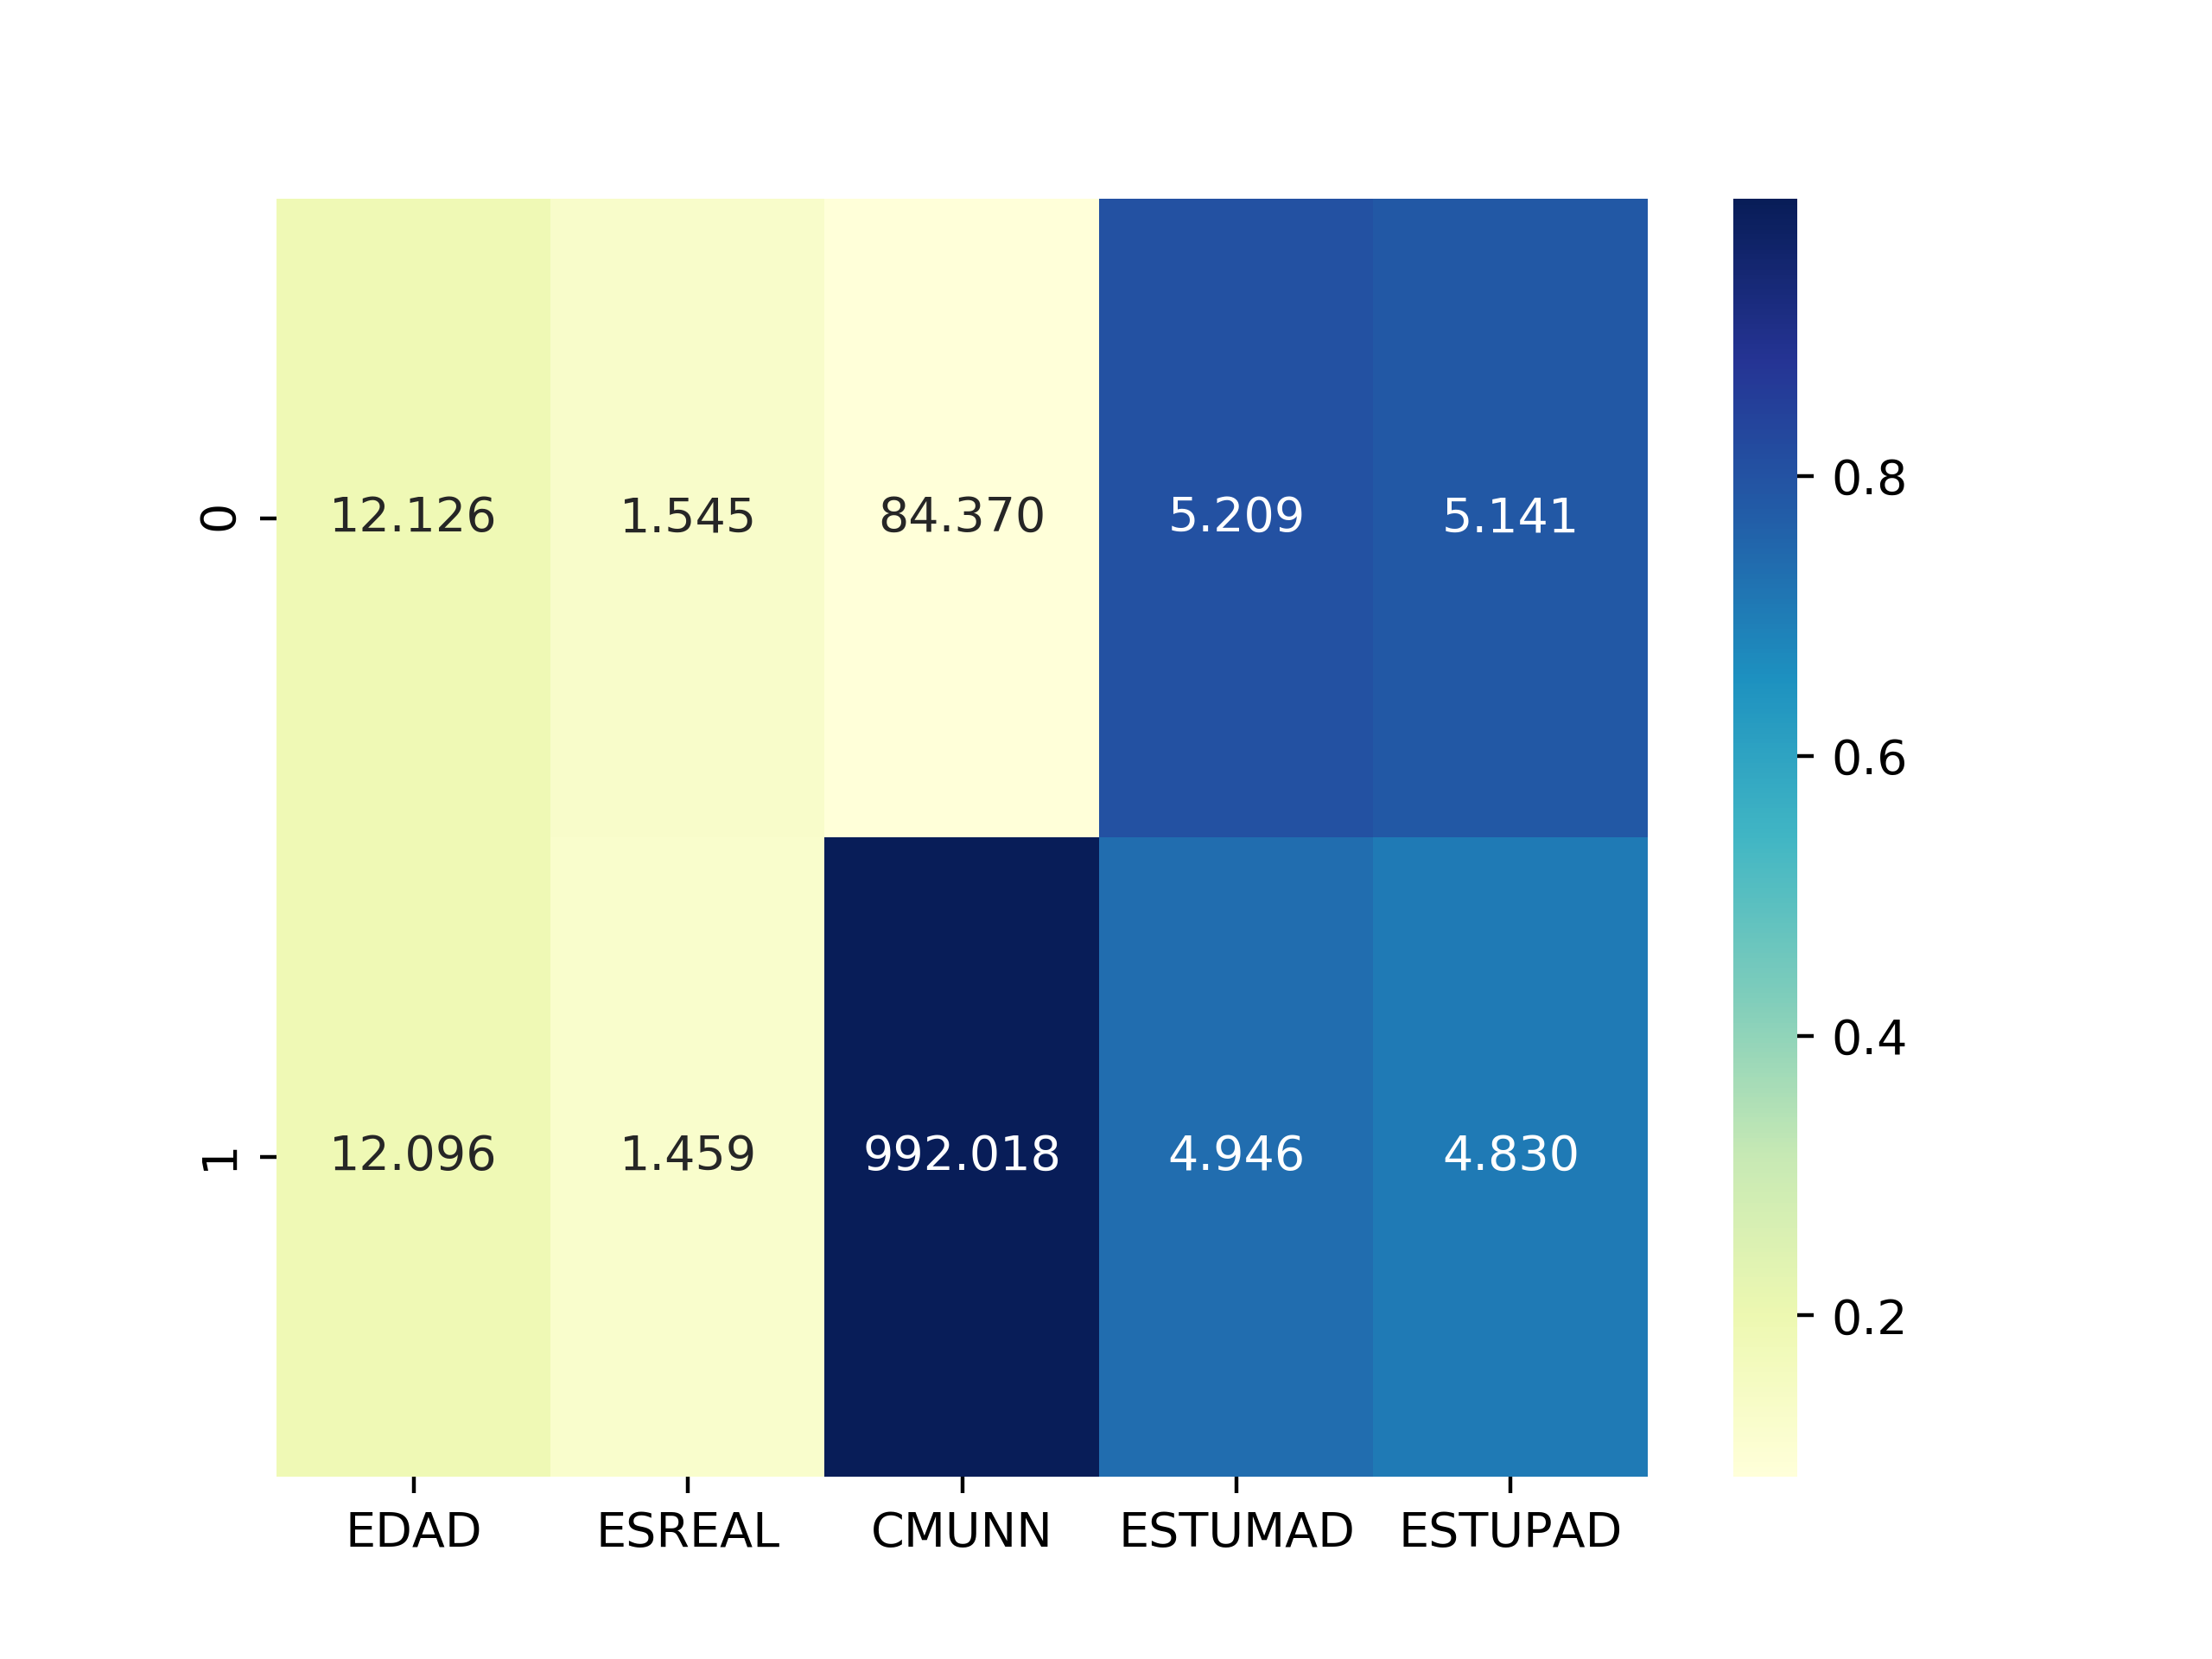
\includegraphics[scale=0.8]{heatmap-ms-1.png}  %el parámetro scale permite agrandar o achicar la imagen. En el nombre de archivo puede especificar directorios
	\caption{Heatmap MeanShift Caso 1} 
	\label{fig:hm-ms-caso1}
\end{figure}

\begin{figure}[H] %con el [H] le obligamos a situar aquí la figura
	\centering
	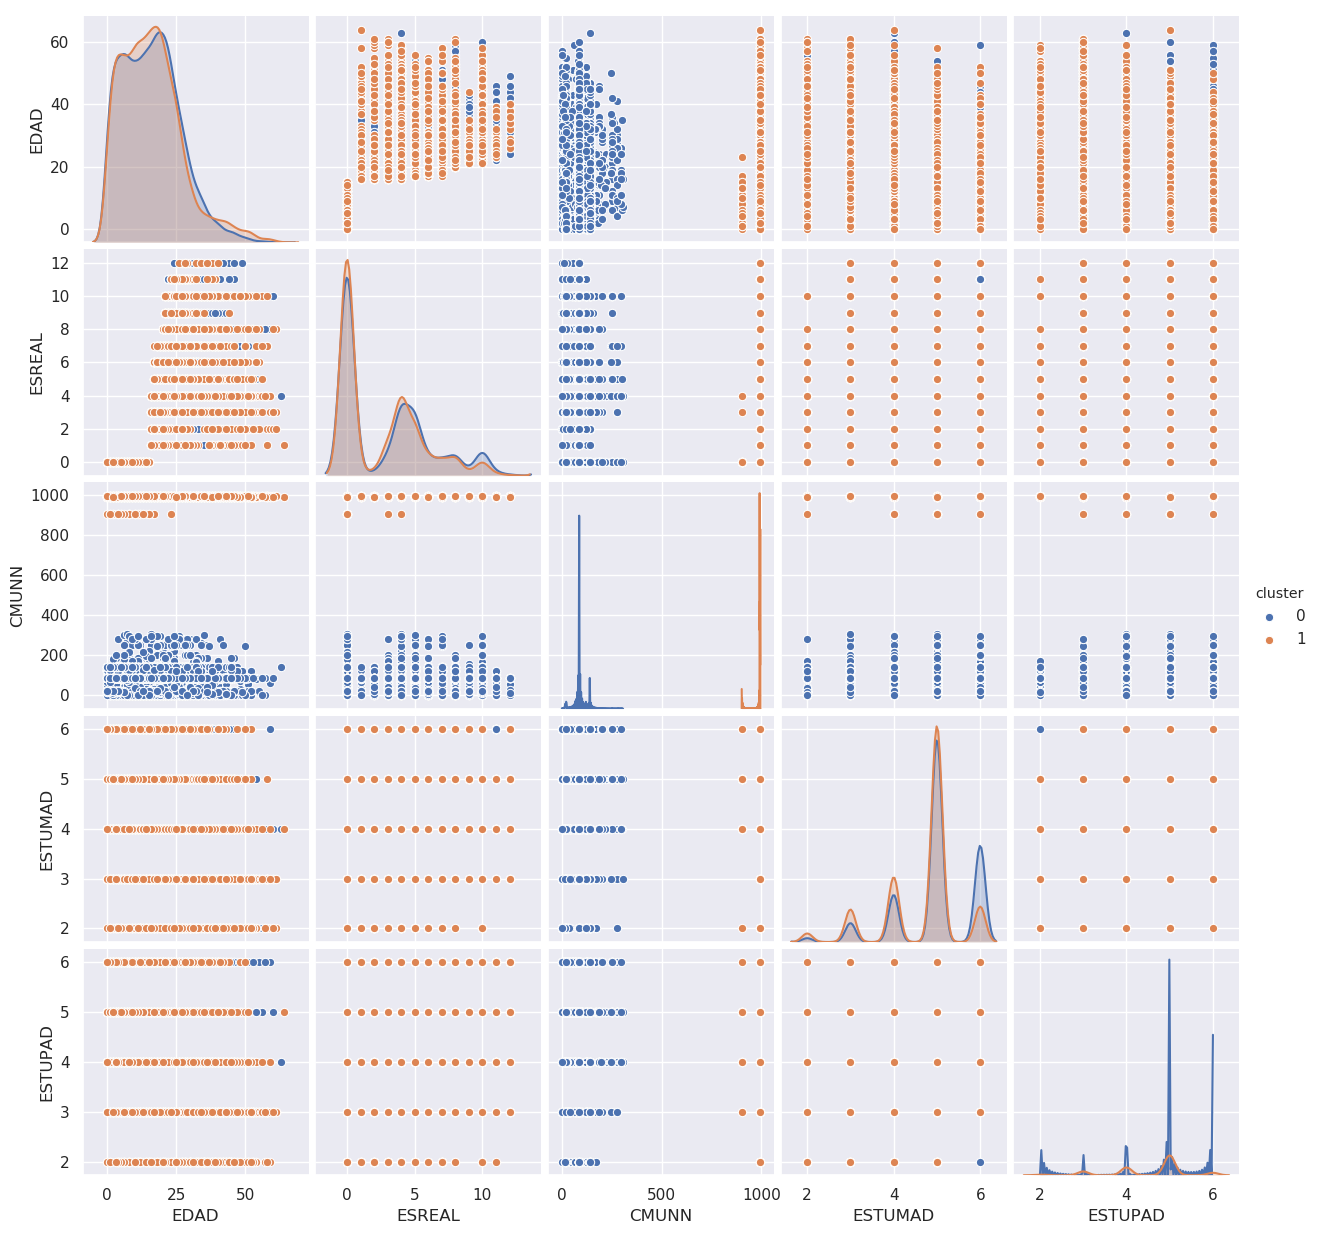
\includegraphics[scale=0.4]{meanshift-1.png}  %el parámetro scale permite agrandar o achicar la imagen. En el nombre de archivo puede especificar directorios
	\caption{Scatter MeanShift Caso 1} 
	\label{fig:sc-ms-caso1}
\end{figure}

Los resultados de MeanShift expresan de nuevo la diferencia entre los lugares donde viven los sujetos. En este caso, los centros de los clusters con respecto a la edad se reducen hasta los 12 años de media y los estudios de los padres en los sujetos con municipio de mayor población tienden a ser mayor. 

\subsection{BIRCH}

BIRCH requiere un número explícito de clusters. A la luz de los algoritmos anteriores, he probado tres configuraciones. Son las siguientes:

\begin{table}[H]
	\begin{tabular}{|c|c|c|c|c|}
		\hline
		Nº Clusters & Tiempo(s) & Silhoutte & Calinski-Harabaz & Tamaño de cada cluster                                                                                                    \\ \hline
		2           & 0.68      & 0.51388   & 24903.026        & \begin{tabular}[c]{@{}c@{}}1: 11690 (54.34\%)\\ 0: 9824 (45.66\%)\end{tabular}                                            \\ \hline
		3           & 0.64      & 0.44622   & 17060.595        & \begin{tabular}[c]{@{}c@{}}0: 11690 (54.34\%)\\ 1:  7386 (34.33\%)\\ 2:  2438 (11.33\%)\end{tabular}                      \\ \hline
		4           & 0.72      & 0.39607   & 17832.861        & \begin{tabular}[c]{@{}c@{}}3:  7386 (34.33\%)\\ 0:  5974 (27.77\%)\\ 1:  5716 (26.57\%)\\ 2:  2438 (11.33\%)\end{tabular} \\ \hline
	\end{tabular}
\end{table}

Vemos de nuevo que el número óptimo de clusters es 2 y que, a medida que crece el número de clusters, las métricas empeoran.

\begin{figure}[H] %con el [H] le obligamos a situar aquí la figura
	\centering
	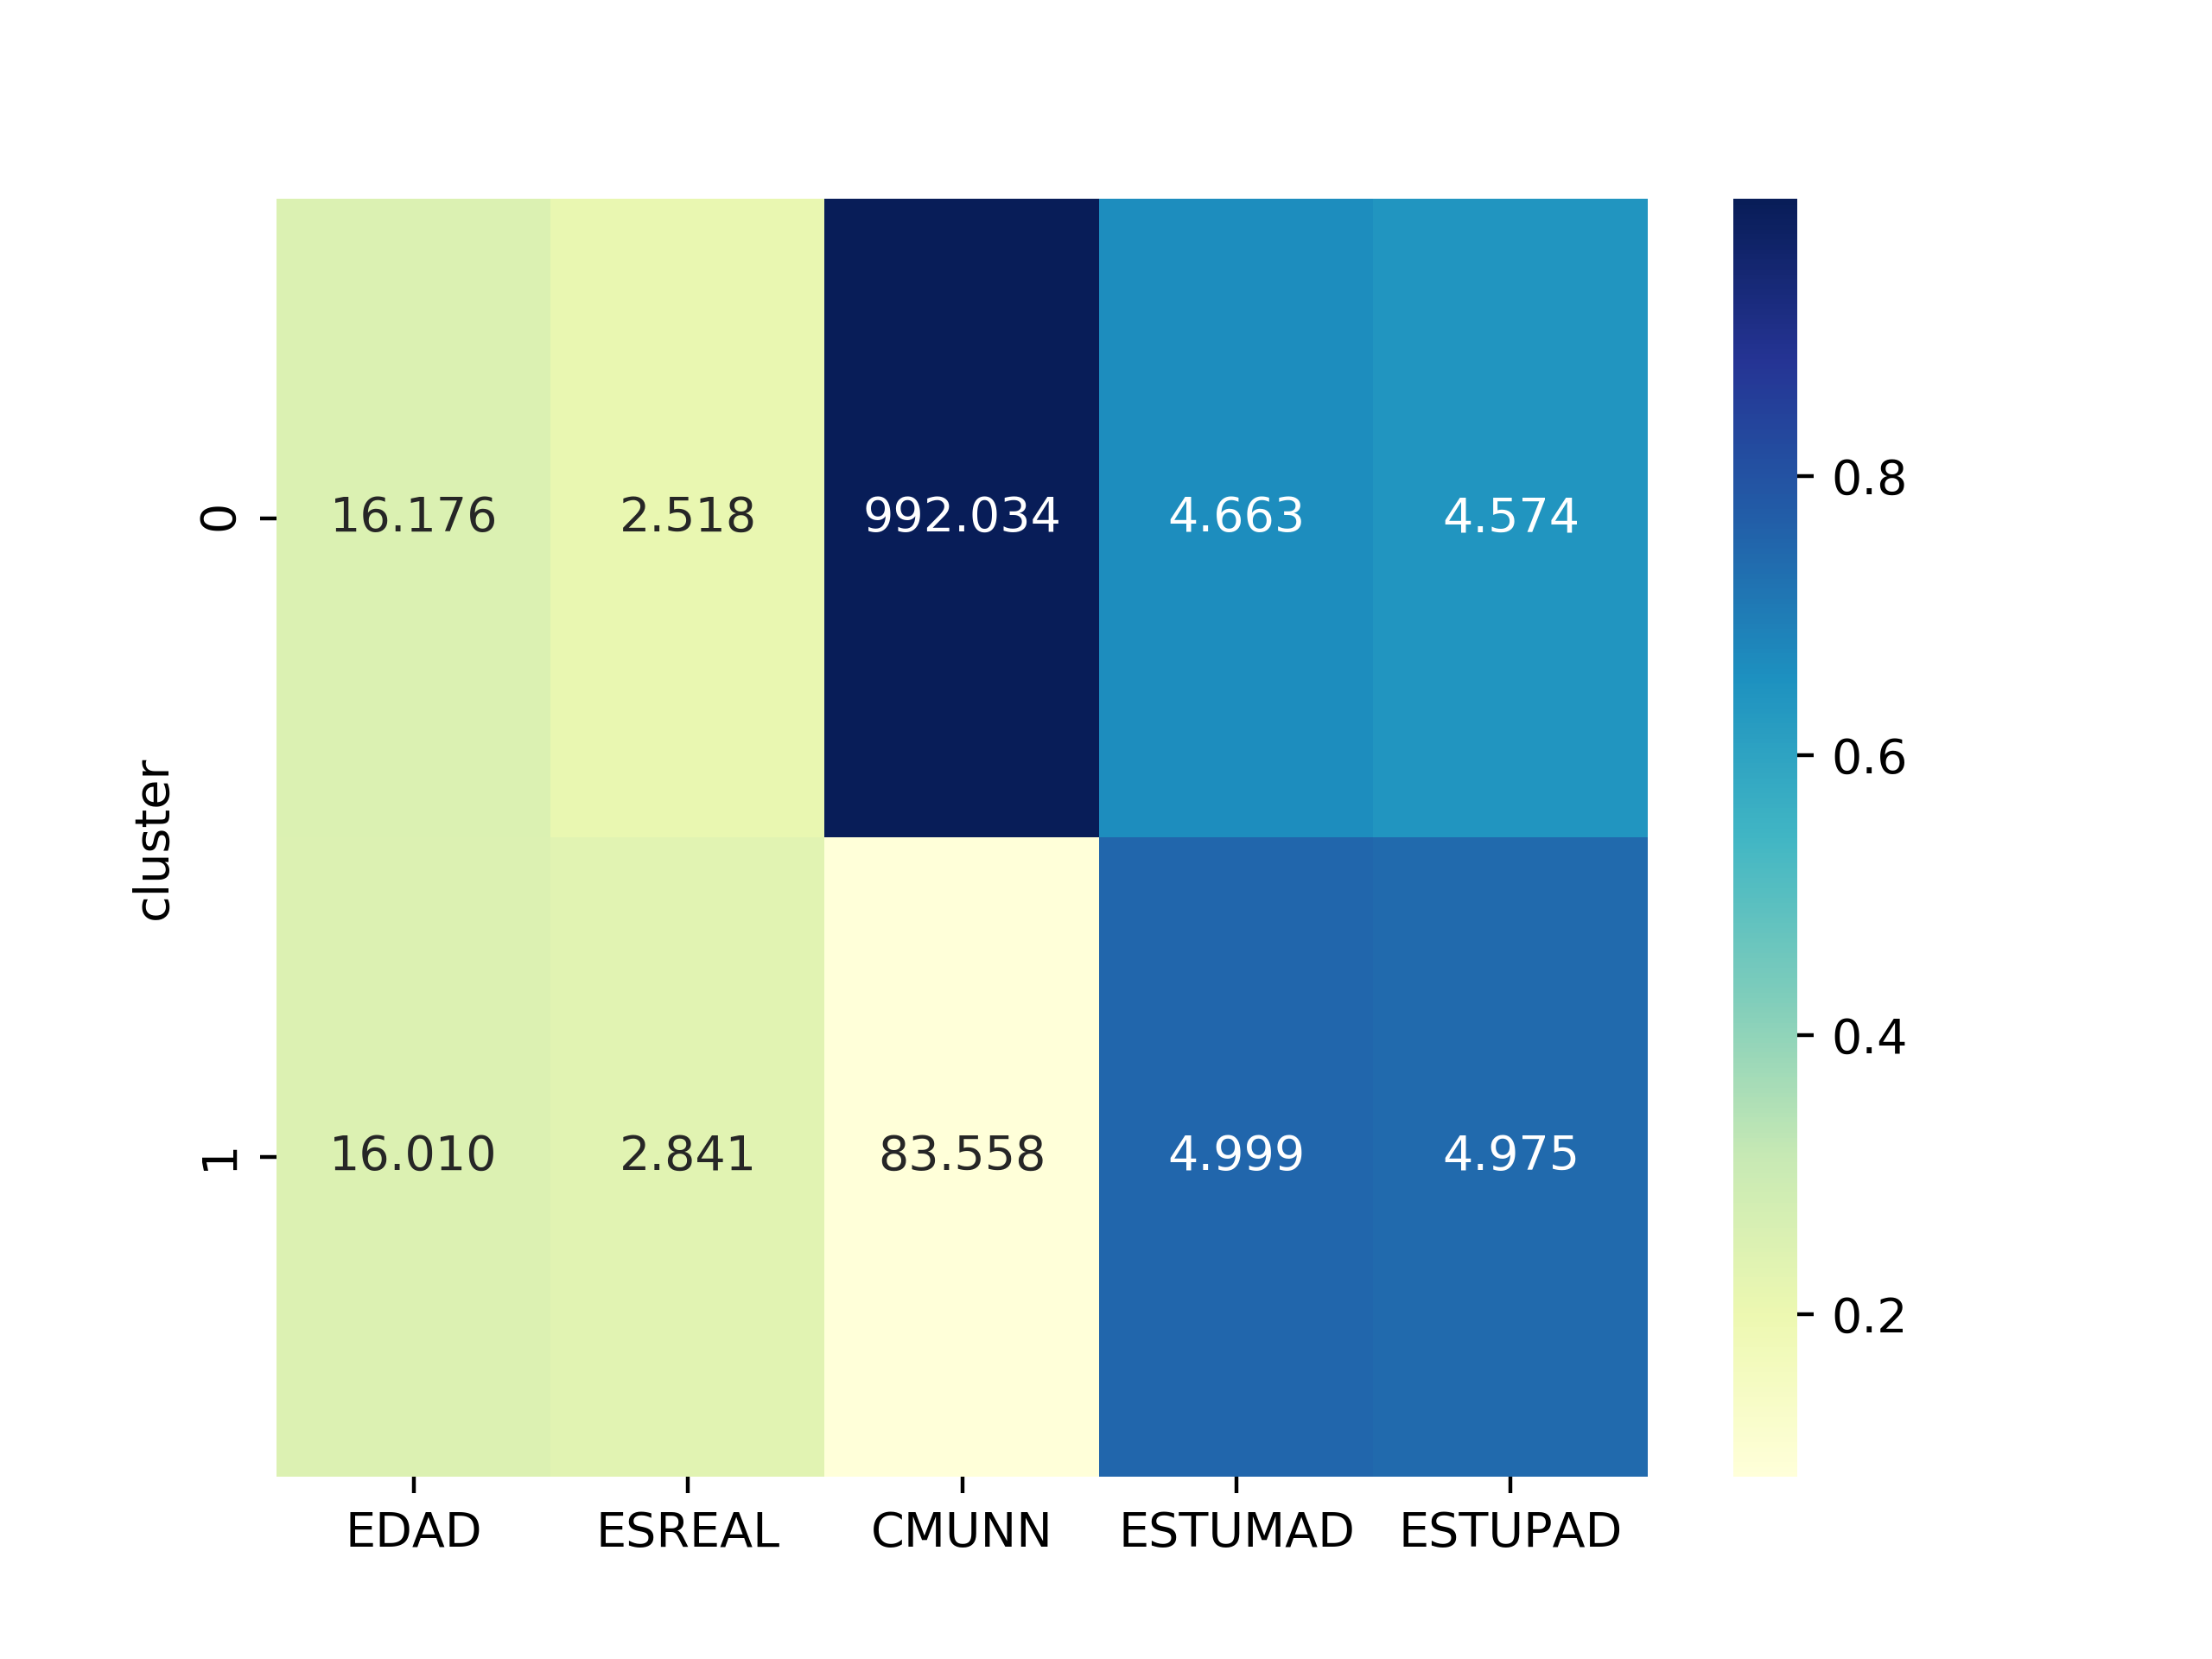
\includegraphics[scale=0.8]{heatmap-br-1.png}  %el parámetro scale permite agrandar o achicar la imagen. En el nombre de archivo puede especificar directorios
	\caption{Heatmap BIRCH Caso 1} 
	\label{fig:hm-br-caso1}
\end{figure}

\begin{figure}[H] %con el [H] le obligamos a situar aquí la figura
	\centering
	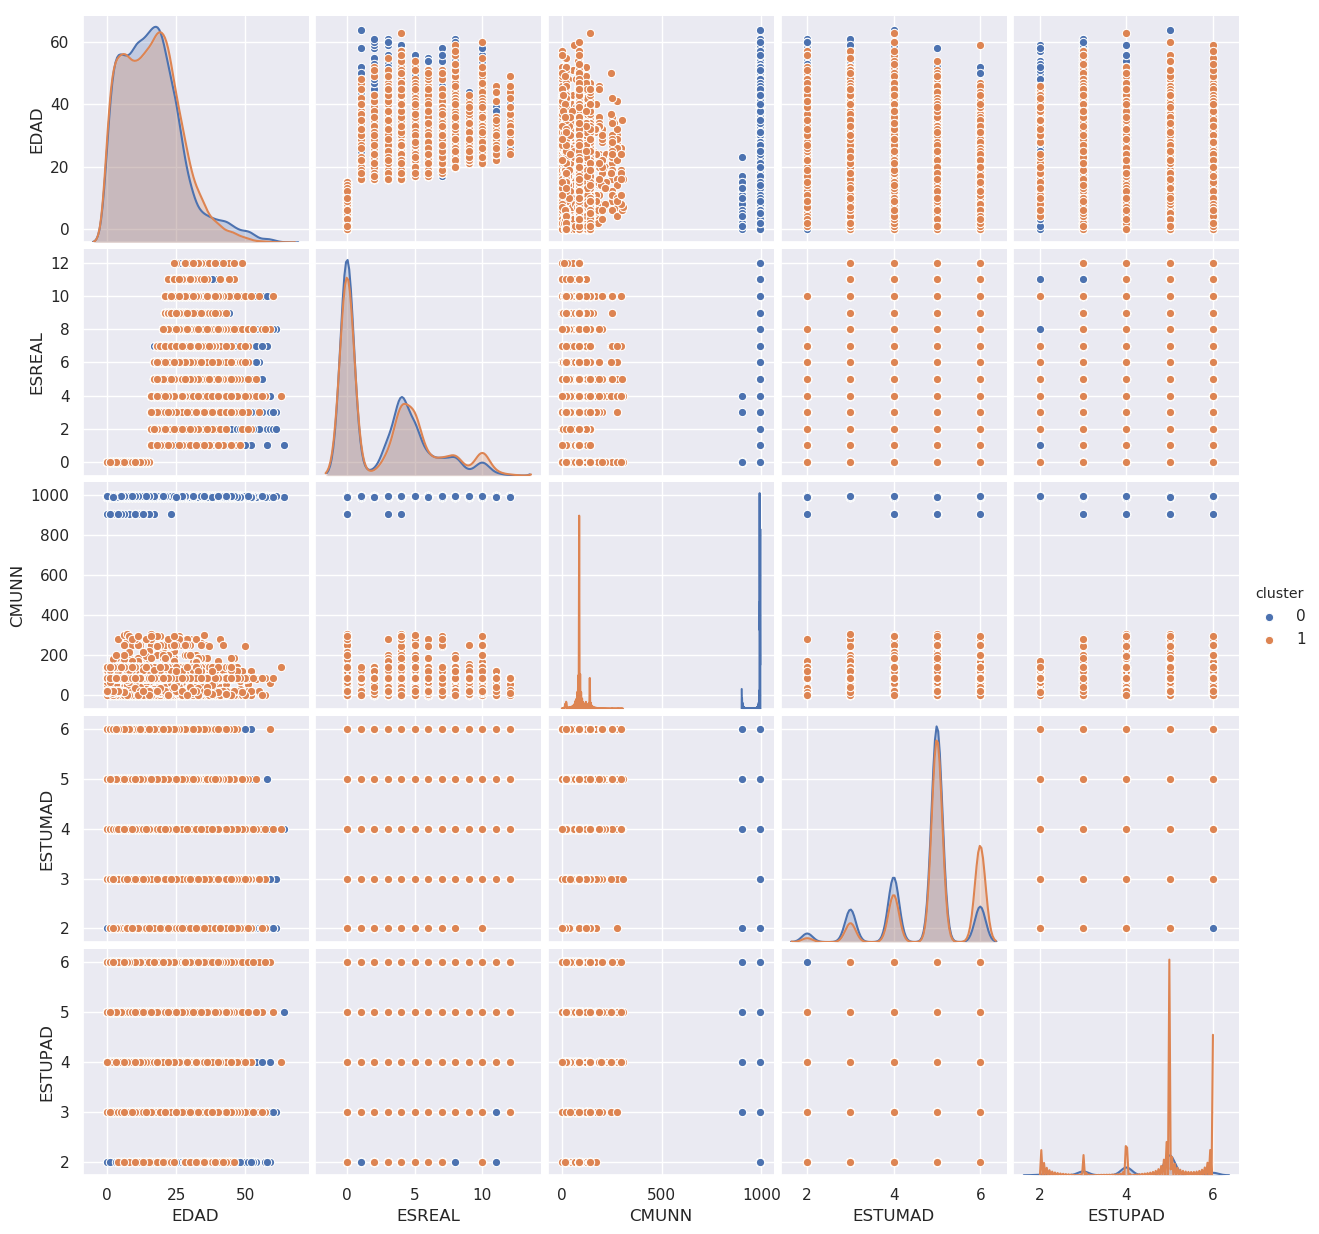
\includegraphics[scale=0.4]{birch-1.png}  %el parámetro scale permite agrandar o achicar la imagen. En el nombre de archivo puede especificar directorios
	\caption{Scatter BIRCH Caso 1} 
	\label{fig:sc-br-caso1}
\end{figure}

Esta ejecución prácticamente calca los resultados de kMeans para 2 clusters, señalando nuevamente la diferencia principal entre el municipio donde habitan los sujetos. Se recupera la edad de 16 años y se iguala de nuevo la formación de los padres.

\subsection{DBSCAN}

DBSCAN necesita dos parámetros, \textit{min\_sampes} (tamaño mínimo) y \textit{eps} (radio). He probado tres configuraciones distintas, teniendo en cuenta que cuanto mayor es el tamaño mínimo o menor el radio la densidad de puntos necesaria para crear un cluster aumenta.

\begin{table}[H]
	\begin{tabular}{|c|c|c|c|c|c|c|}
		\hline
		Nº Clusters & T (s) & Epsilon & Min\_Samples & Silhoutte & Calinski-Harabaz & Tamaño                                                                                                                                                                                                                                                                                                                                                                                                                                                                                                                                                                                                                  \\ \hline
		2           & 2.67  & 0.3     & 10           & 0.51388   & 12460.563        & \begin{tabular}[c]{@{}c@{}}1: 11689 (54.33\%)\\ 0:  9821 (45.65\%)\\ -1:     4 ( 0.02\%)\end{tabular}                                                                                                                                                                                                                                                                                                                                                                                                                                                                                                 \\ \hline
		3           & 1.95  & 0.25    & 10           & 0.41986   & 8357.047         & \begin{tabular}[c]{@{}c@{}}1: 11631 (54.06\%)\\ 0:  9791 (45.51\%)\\ -1:    78 ( 0.36\%)\\ 2:    14 ( 0.07\%)\end{tabular}                                                                                                                                                                                                                                                                                                                                                                                                                                                                                              \\ \hline
		25          & 1.95  & 0.2     & 50           & 0.13990   & 2298.908         & \begin{tabular}[c]{@{}c@{}}4:  4681 (21.76\%)\\ 3:  4401 (20.46\%)\\ 7:  1948 ( 9.05\%)\\ -1:  1110 ( 5.16\%)\\ 10:  1071 ( 4.98\%)\\ 16:  1031 ( 4.79\%)\\ 8:   920 ( 4.28\%)\\ 13:   817 ( 3.80\%)\\ 12:   771 ( 3.58\%)\\ 1:   688 ( 3.20\%)\\ 2:   603 ( 2.80\%)\\ 14:   589 ( 2.74\%)\\ 5:   586 ( 2.72\%)\\ 21:   519 ( 2.41\%)\\ 9:   280 ( 1.30\%)\\ 19:   277 ( 1.29\%)\\ 23:   255 ( 1.19\%)\\ 0:   175 ( 0.81\%)\\ 18:   154 ( 0.72\%)\\ 15:   115 ( 0.53\%)\\ 6:   105 ( 0.49\%)\\ 22:   104 ( 0.48\%)\\ 11:    97 ( 0.45\%)\\ 17:    96 ( 0.45\%)\\ 24:    63 ( 0.29\%)\\ 20:    58 ( 0.27\%)\end{tabular} \\ \hline
	\end{tabular}
\end{table}

Sus representaciones gráficas, en el caso de 2 clusters, son:

\begin{figure}[H] %con el [H] le obligamos a situar aquí la figura
	\centering
	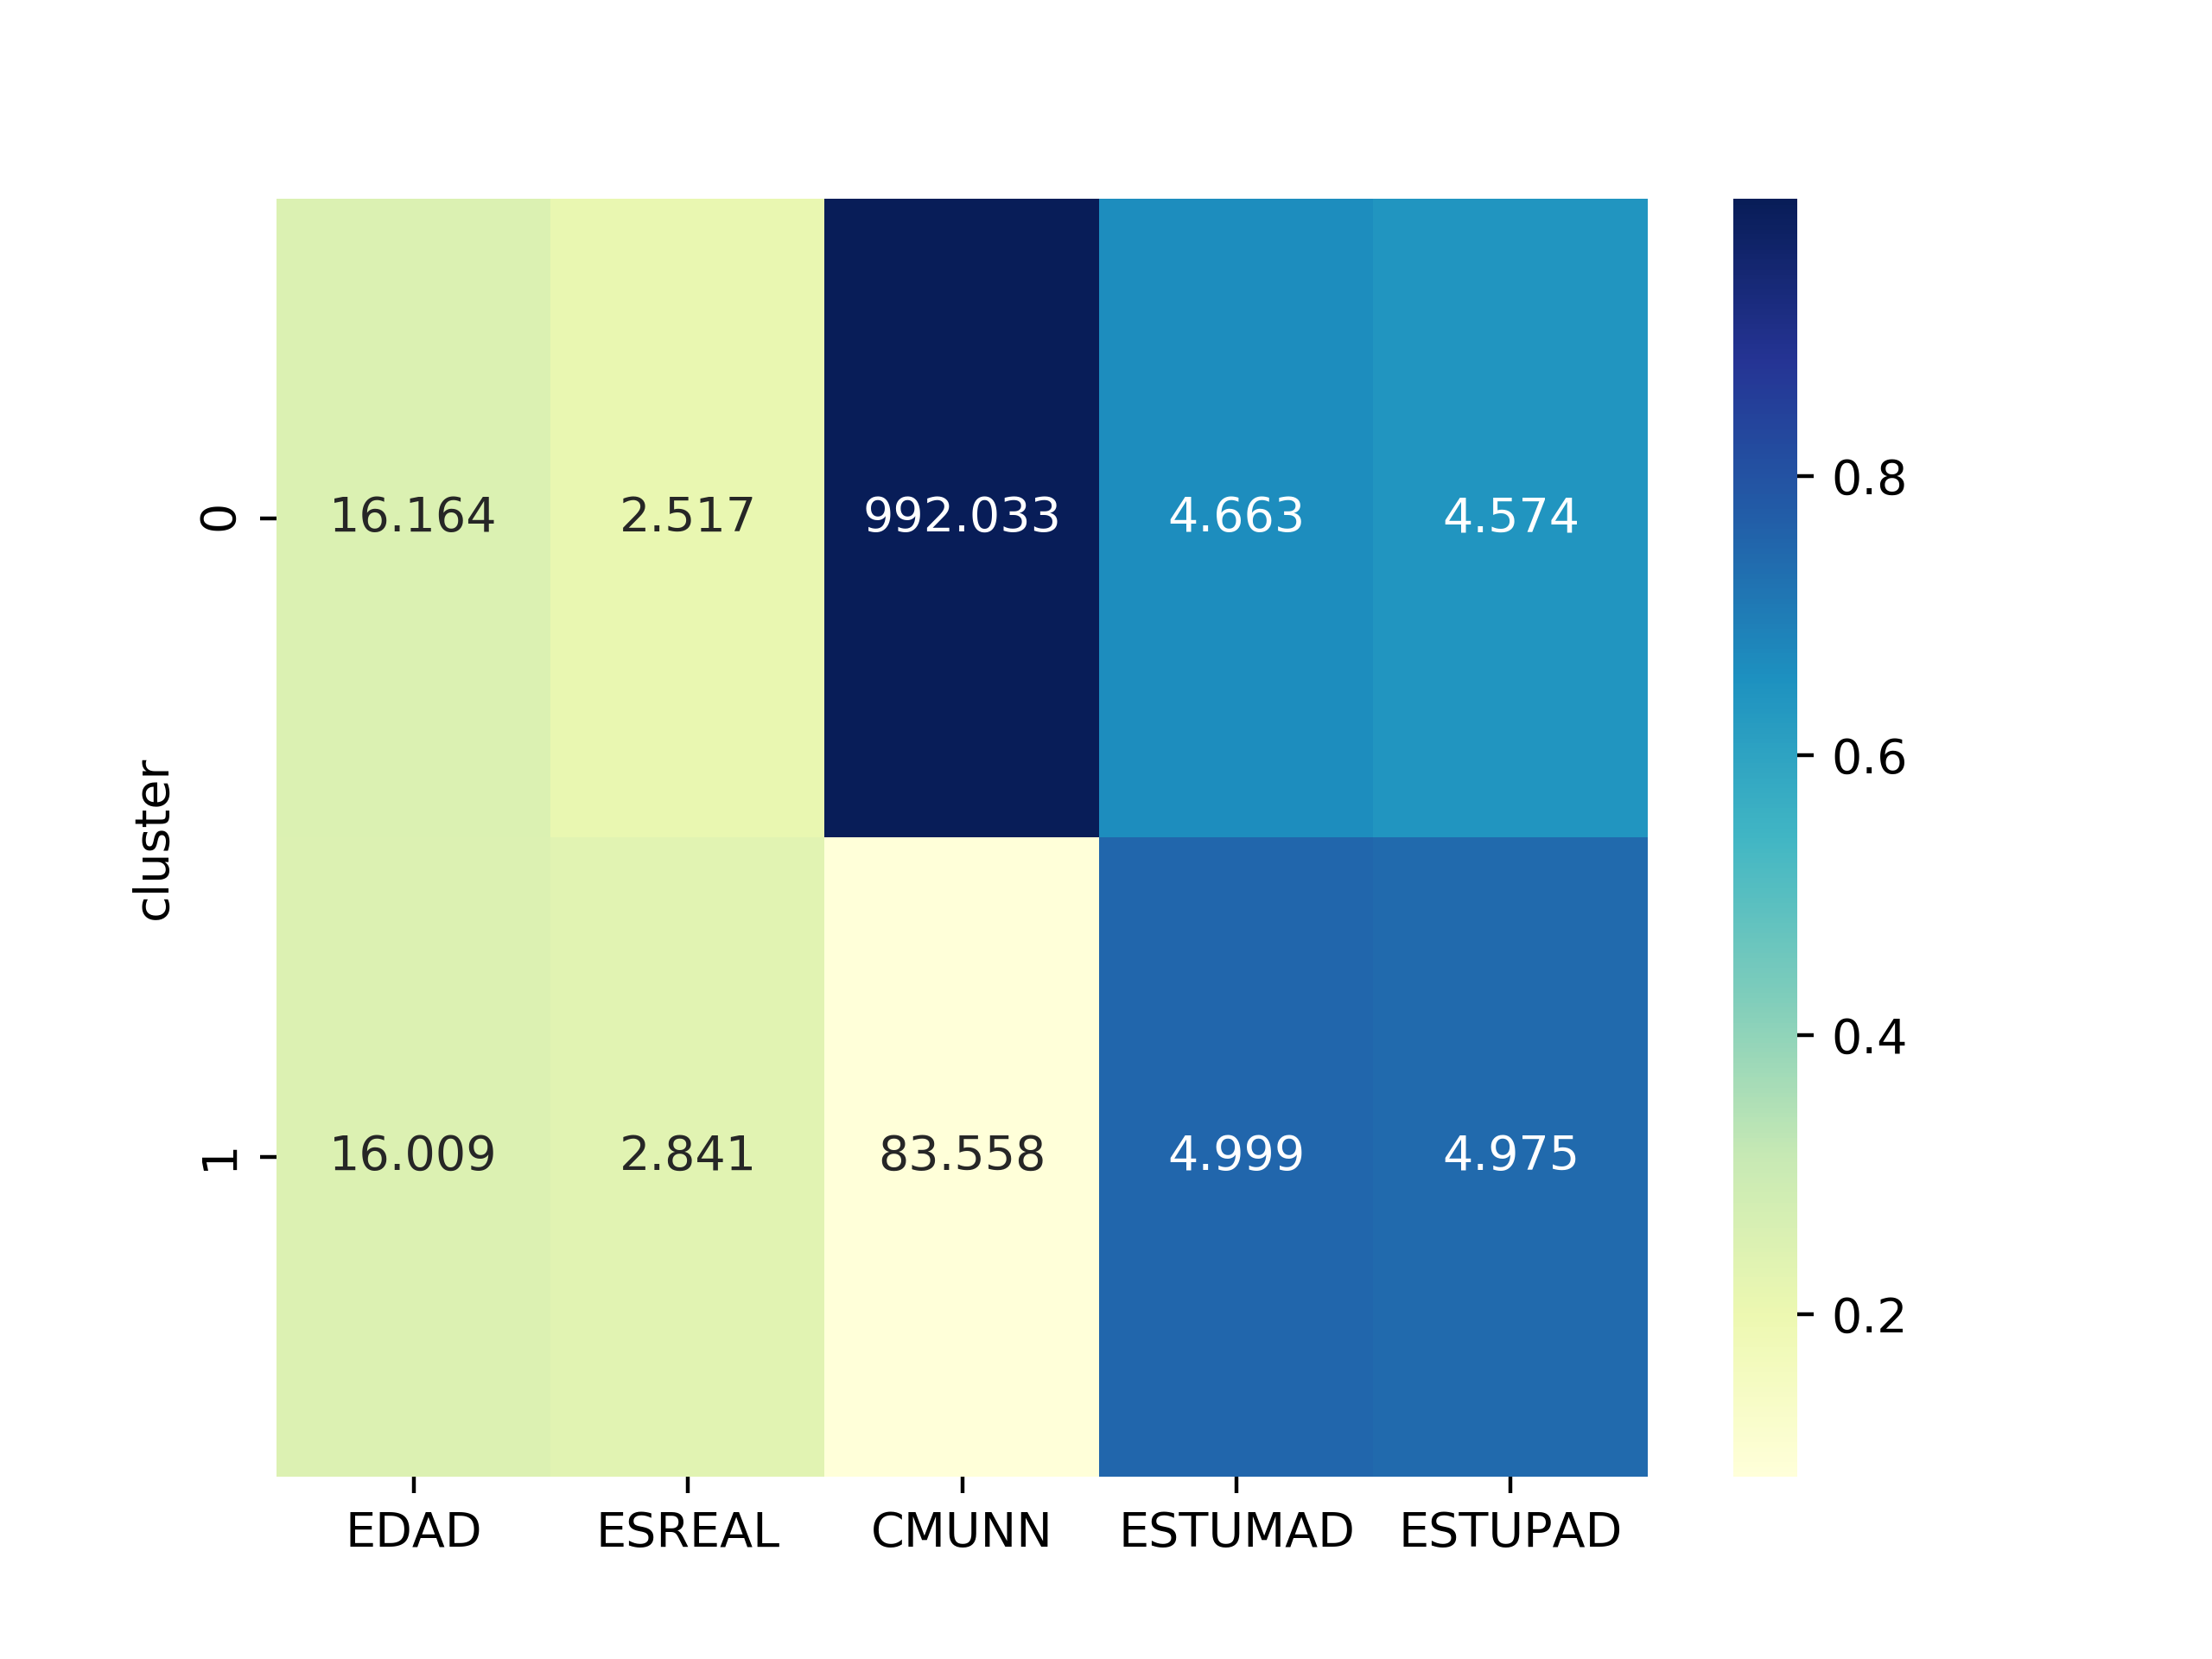
\includegraphics[scale=0.5]{heatmap-dbscan1.png}  %el parámetro scale permite agrandar o achicar la imagen. En el nombre de archivo puede especificar directorios
	\caption{Heatmap DBSCAN Caso 1} 
	\label{fig:hm-db-caso1}
\end{figure}

\begin{figure}[H] %con el [H] le obligamos a situar aquí la figura
	\centering
	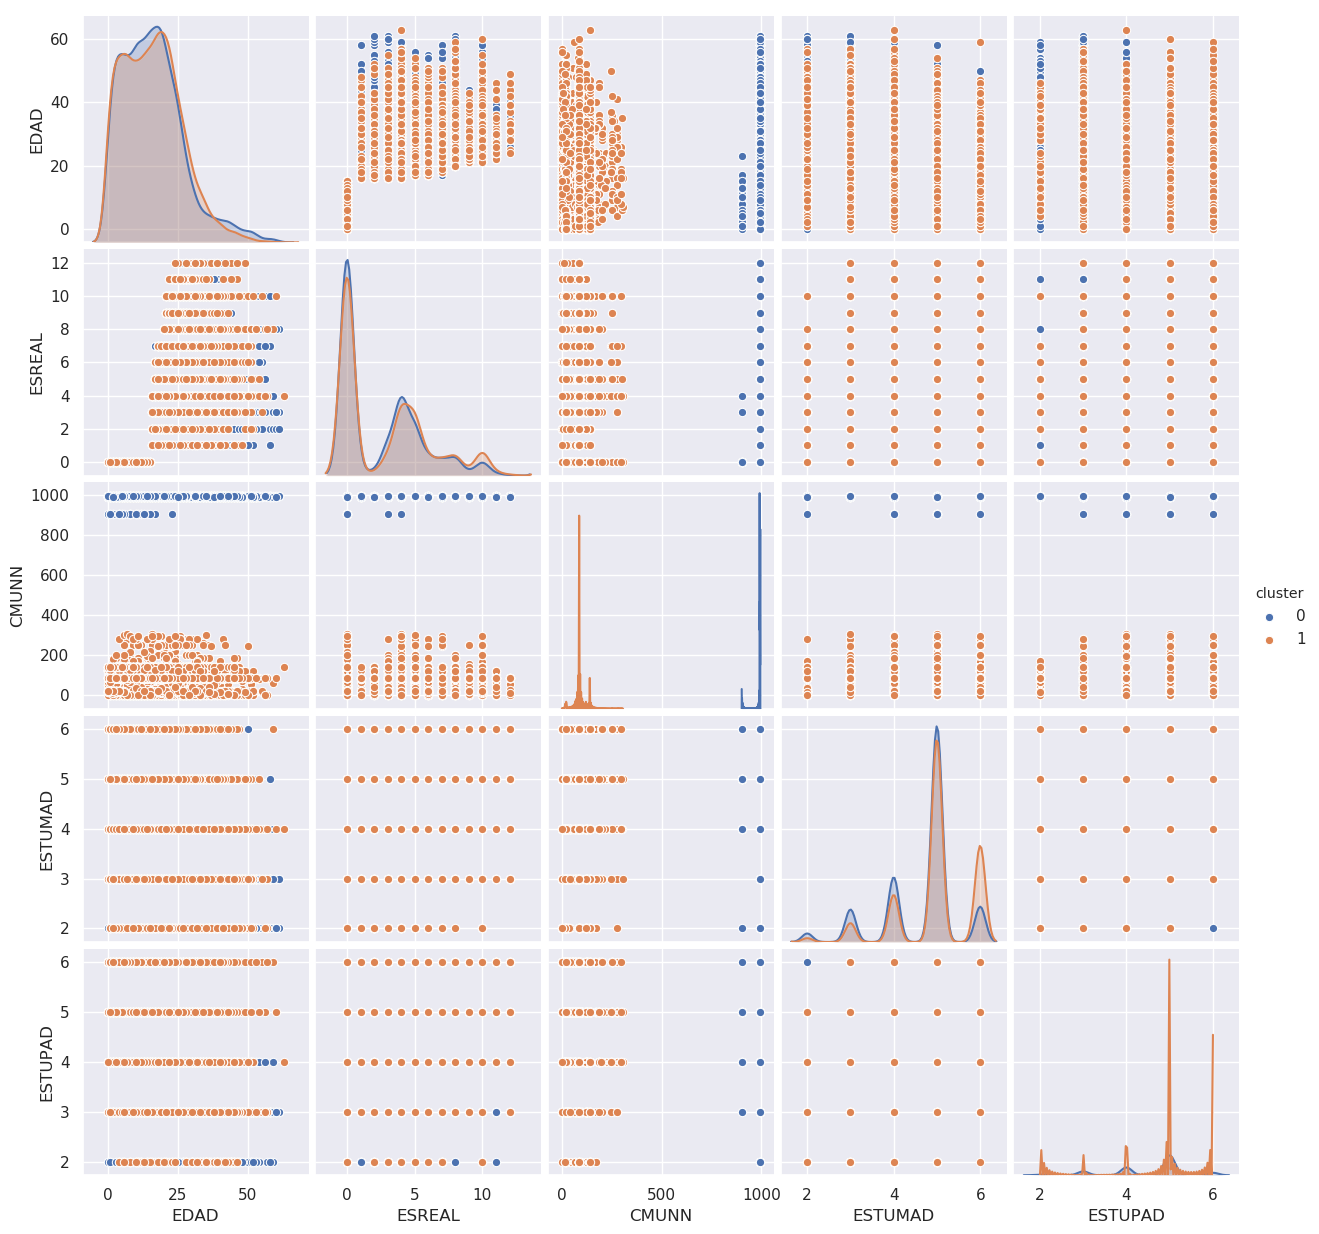
\includegraphics[scale=0.37]{dbscan1.png}  %el parámetro scale permite agrandar o achicar la imagen. En el nombre de archivo puede especificar directorios
	\caption{Scatter DBSCAN Caso 1} 
	\label{fig:sc-db-caso1}
\end{figure}

Como se aprecia, los resultados son totalmente análogos a los comentados anteriormente.

\subsection{Aglomerativo}

Para enfrentarme al algoritmo de cluster jerárquico aglomerativo con estrategia Ward (de la misma forma en todos los casos), evalúo el algoritmo en 100 clusters para eliminar outliers. A continuación, obviando la columna de cluster pronosticada, dibujo el dendograma.

\begin{figure}[H] %con el [H] le obligamos a situar aquí la figura
	\centering
	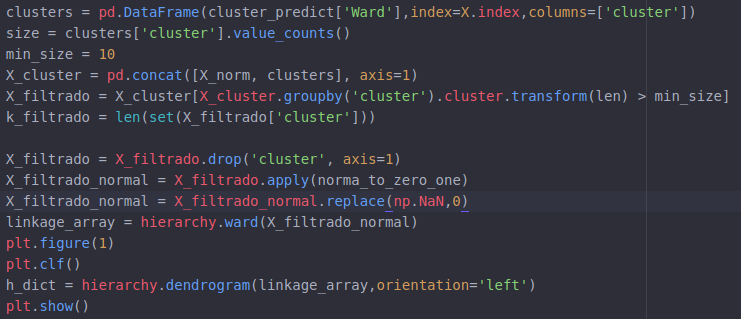
\includegraphics[scale=0.5]{capt2.png}  %el parámetro scale permite agrandar o achicar la imagen. En el nombre de archivo puede especificar directorios
	\label{fig:conf2}
\end{figure}


 En función del dendograma elijo el número real de clusters. Aunque es algo difusa, la idea es general: minimizar la distancia intracluster y maximizar la distancia intercluster. Además, hay que tener en cuenta que si el número de instancias es mayor que 1000, cojo una muestra de 1000 para garantizar que el algoritmo sea eficiente y acabe. Este es el resultado:

\begin{figure}[H] %con el [H] le obligamos a situar aquí la figura
	\centering
	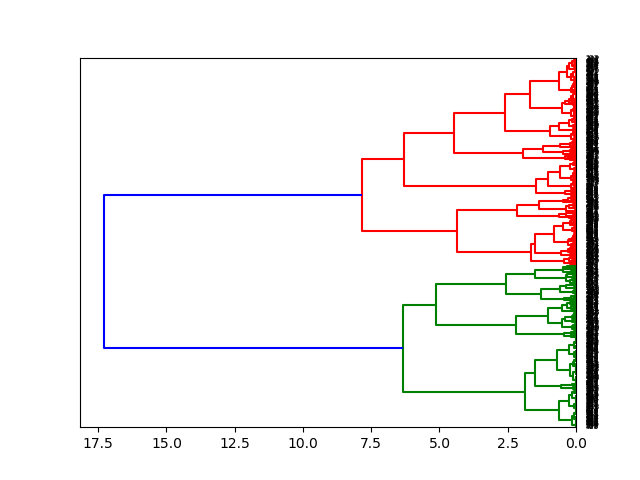
\includegraphics[scale=0.5]{dendograma1.png}  %el parámetro scale permite agrandar o achicar la imagen. En el nombre de archivo puede especificar directorios
	\caption{Dendograma cluster jerárquico Caso 1} 
	\label{fig:dendogram-caso1}
\end{figure}

A raíz de esa imagen, elijo 5 clusters.

\begin{table}[H]
	\begin{tabular}{|c|c|c|}
		\hline
		Nº Clusters & Tiempo(s) & Tamaño de los clusters                                                                                                                         \\ \hline
		5           & 0.03      & \begin{tabular}[c]{@{}c@{}}0:   274 (27.40\%)\\ 3:   250 (25.00\%)\\ 1:   215 (21.50\%)\\ 2:   158 (15.80\%)\\ 4:   103 (10.30\%)\end{tabular} \\ \hline
	\end{tabular}
\end{table}


A partir de aquí se genera el heatmap:

\begin{figure}[H] %con el [H] le obligamos a situar aquí la figura
	\centering
	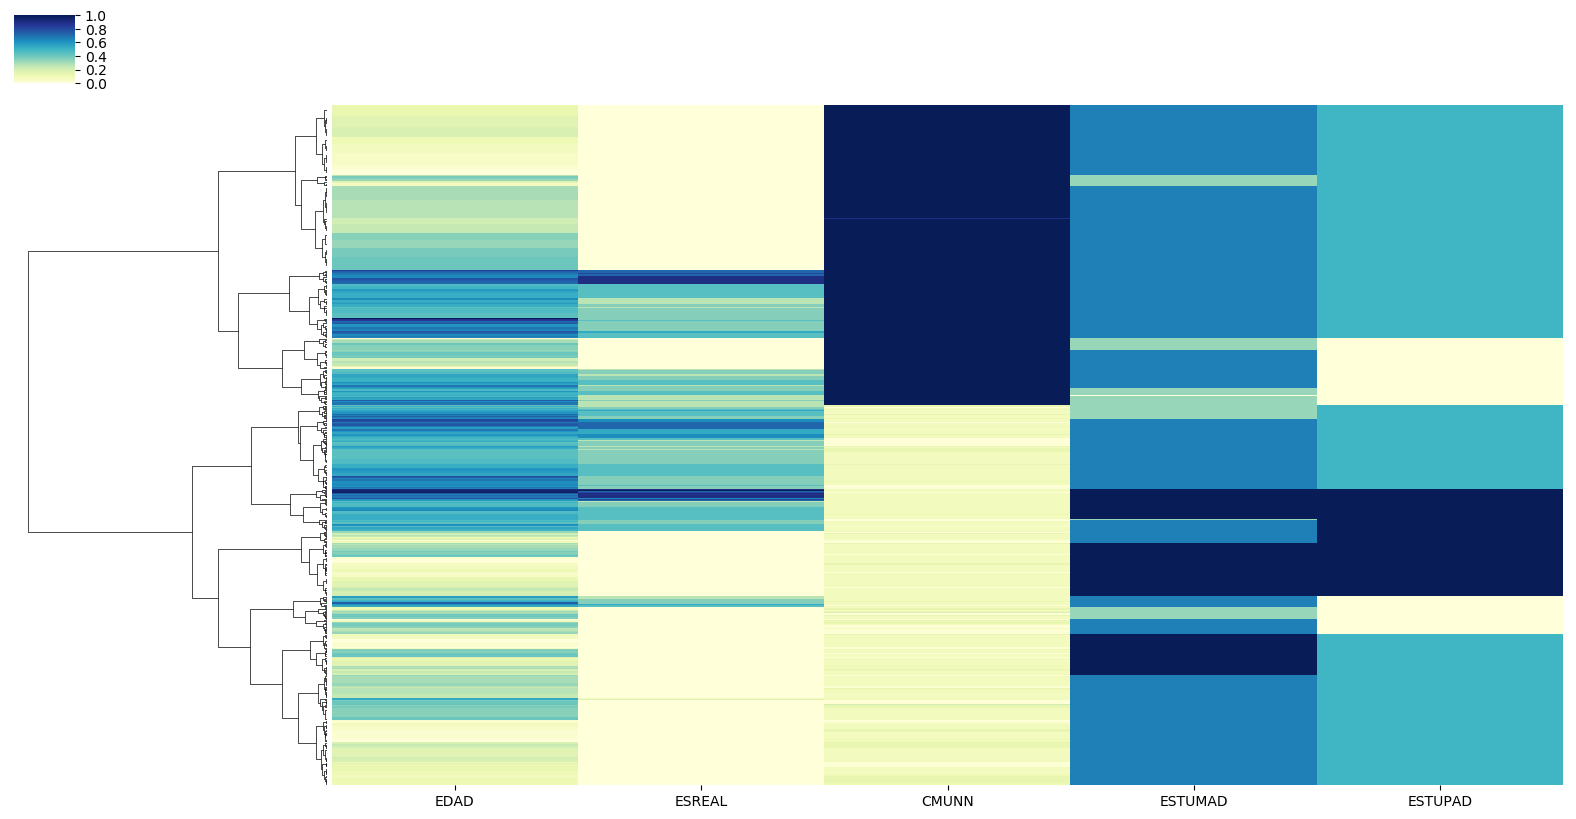
\includegraphics[scale=0.4]{clustermap1.png}  %el parámetro scale permite agrandar o achicar la imagen. En el nombre de archivo puede especificar directorios
	\caption{Clustermap cluster jerárquico Caso 1} 
	\label{fig:clustermap-caso1}
\end{figure}

\begin{figure}[H] %con el [H] le obligamos a situar aquí la figura
	\centering
	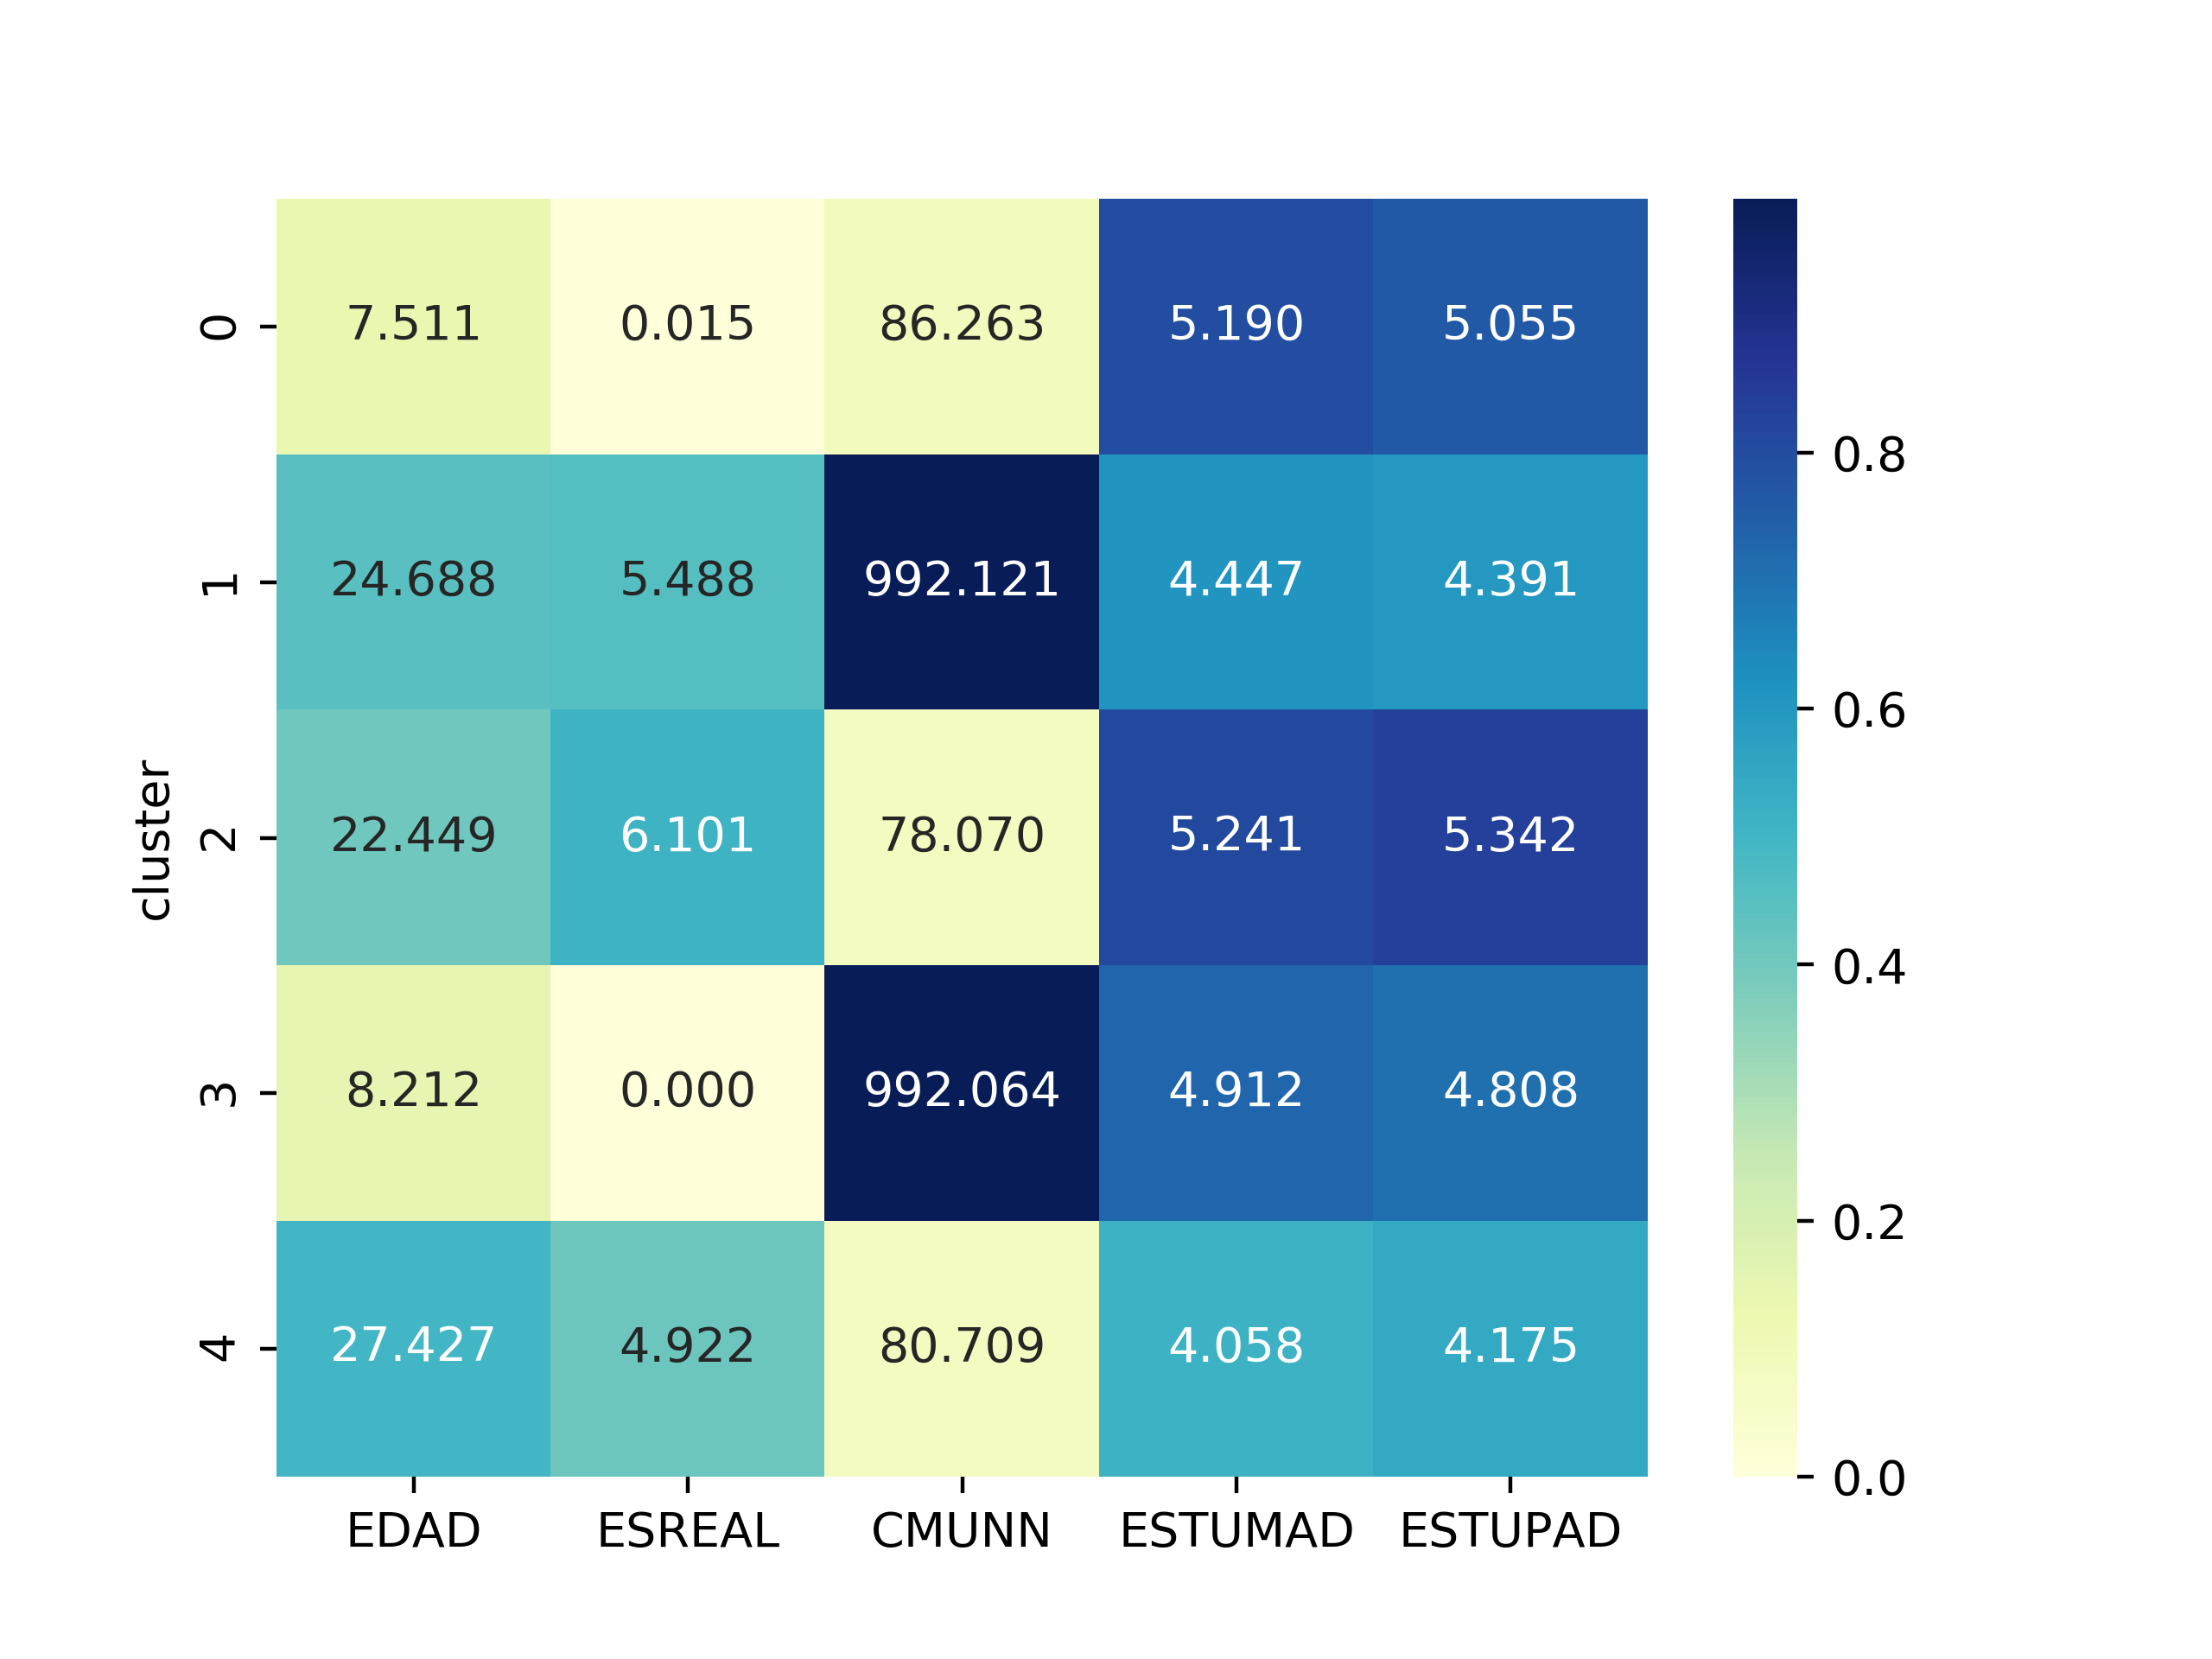
\includegraphics[scale=0.7]{heatmap-jerarquico1.png}  %el parámetro scale permite agrandar o achicar la imagen. En el nombre de archivo puede especificar directorios
	\caption{Heatmap cluster jerárquico Caso 1} 
	\label{fig:heatmapj-caso1}
\end{figure}

Como consecuencia de la creación de 5 clusters, se pueden observar subgrupos dentro los que ya conocíamos. Por ejemplo, encontramos individuos de 24 años con bachillerato que viven aún con sus padres en zonas con pocos habitantes. Obviamente los niños de 8 años también lo hacen. Por otra parte, en zonas con muchos habitantes encontramos individuos con 22 años con una formación más alta (formación profesional media) y otros que aún con 27 siguen cohabitando con sus progenitores. En todos los casos los padres tienen una formación parecida (entorno al bachillerato). Este tipo de estudios da pie a investigar otros factores, por ejemplo, el acuciante precio del alquiler en las ciudades, que impide a los jóvenes con pocos recursos independizarse.

\subsection{Interpretación de la segmentación}

A la luz de los resultados de los distintos algoritmos, podemos concluir que los individuos que aún viven con sus padres en la provincia de Granada son, por lo general, menores de 25 años (con ciertas excepciones captadas en el clustering jerárquico) y se suelen dividir en dos grandes grupos: sujetos que habitan en un municipio de entre 2000 y 5000 habitantes o en un municipio bastante más poblado del cual sólo conocemos su código (alrededor de 90). La formación del sujeto suele ser media-baja, nunca llegando a la universitaria, al igual que la de sus padres. Un estudio más profundo del municipio en cuestión nos aclararía exacta hay en esos lugares. En cuanto a un análisis más técnico, los mejores valores de métricas se dan para dos clusters llegando a Silhouette del 0.51388 y Calinski-Harabaz de hasta 25000.

\section{Caso de estudio 2: Mujeres ingenieras}

Me dispongo ahora a analizar la situación de las mujeres científicas en la provincia de Granada. Para ello, impongo que \textit{SEXO == 6} y \textit{TESTUD==5}. Además, utilizo las características siguientes:
\begin{itemize}
	\item EDAD
	\item CMUNN
	\item CODTRABA
	\item TDESP
	\item ESTUCON
\end{itemize}


\begin{figure}[H] %con el [H] le obligamos a situar aquí la figura
	\centering
	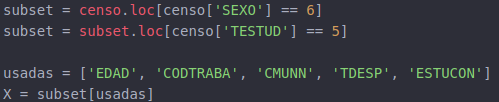
\includegraphics[scale=0.7]{capt3.png}  %el parámetro scale permite agrandar o achicar la imagen. En el nombre de archivo puede especificar directorios
	\caption{Configuración caso 2} 
	\label{fig:conf-caso2}
\end{figure}

He de señalar que este caso tiene un tamaño muy reducido (430 instancias), lo que indica la situación de la ingeniería/arquitectura en 2011 con respecto a la mujer en Granada.
\subsection{kMeans}

\begin{figure}[H] %con el [H] le obligamos a situar aquí la figura
	\centering
	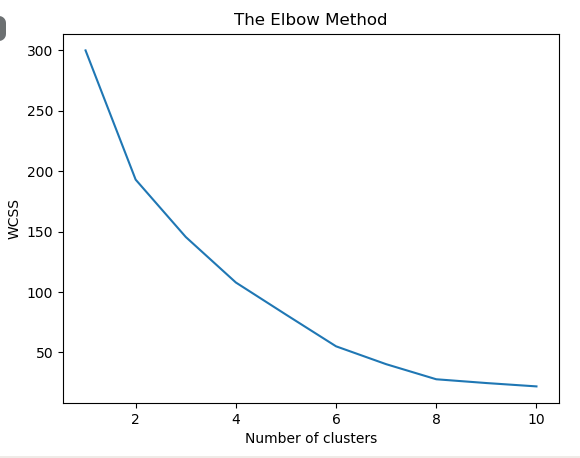
\includegraphics[scale=0.5]{em-2.png}  %el parámetro scale permite agrandar o achicar la imagen. En el nombre de archivo puede especificar directorios
	\caption{Elbow Method caso 2} 
	\label{fig:em-caso2}
\end{figure}

Elbow Method nos indica que el mejor valor de k es 8. No obstante, pruebo 3 configuraciones distintas, correspondientes a los tres picos que se ven en la gráfica (k=2, k=6 y k=8).

\begin{table}[]
	\begin{tabular}{|c|c|c|c|c|}
		\hline
		Nº Clusters & Tiempo(s) & Tamaño de los clusters                                                                                                                                                                                        & Silhouette & Calinski-Harabaz \\ \hline
		2           & 0.02      & \begin{tabular}[c]{@{}c@{}}1:   219 (50.93\%)\\ 0:   211 (49.07\%)\end{tabular}                                                                                                                               & 0.36921    & 237.128          \\ \hline
		6           & 0.04      & \begin{tabular}[c]{@{}c@{}}4:    92 (21.40\%)\\ 0:    75 (17.44\%)\\ 5:    73 (16.98\%)\\ 1:    72 (16.74\%)\\ 3:    63 (14.65\%)\\ 2:    55 (12.79\%)\end{tabular}                                           & 0.58784    & 377.099          \\ \hline
		8           & 0.04      & \begin{tabular}[c]{@{}c@{}}0:    92 (21.40\%)\\ 6:    75 (17.44\%)\\ 1:    63 (14.65\%)\\ 3:    55 (12.79\%)\\ 5:    38 ( 8.84\%)\\ 4:    36 ( 8.37\%)\\ 2:    36 ( 8.37\%)\\ 7:    35 ( 8.14\%)\end{tabular} & 0.68604    & 590.209          \\ \hline
	\end{tabular}
\end{table}

Se hace por tanto evidente la conveniencia de elegir 8 clusters.

\begin{figure}[H] %con el [H] le obligamos a situar aquí la figura
	\centering
	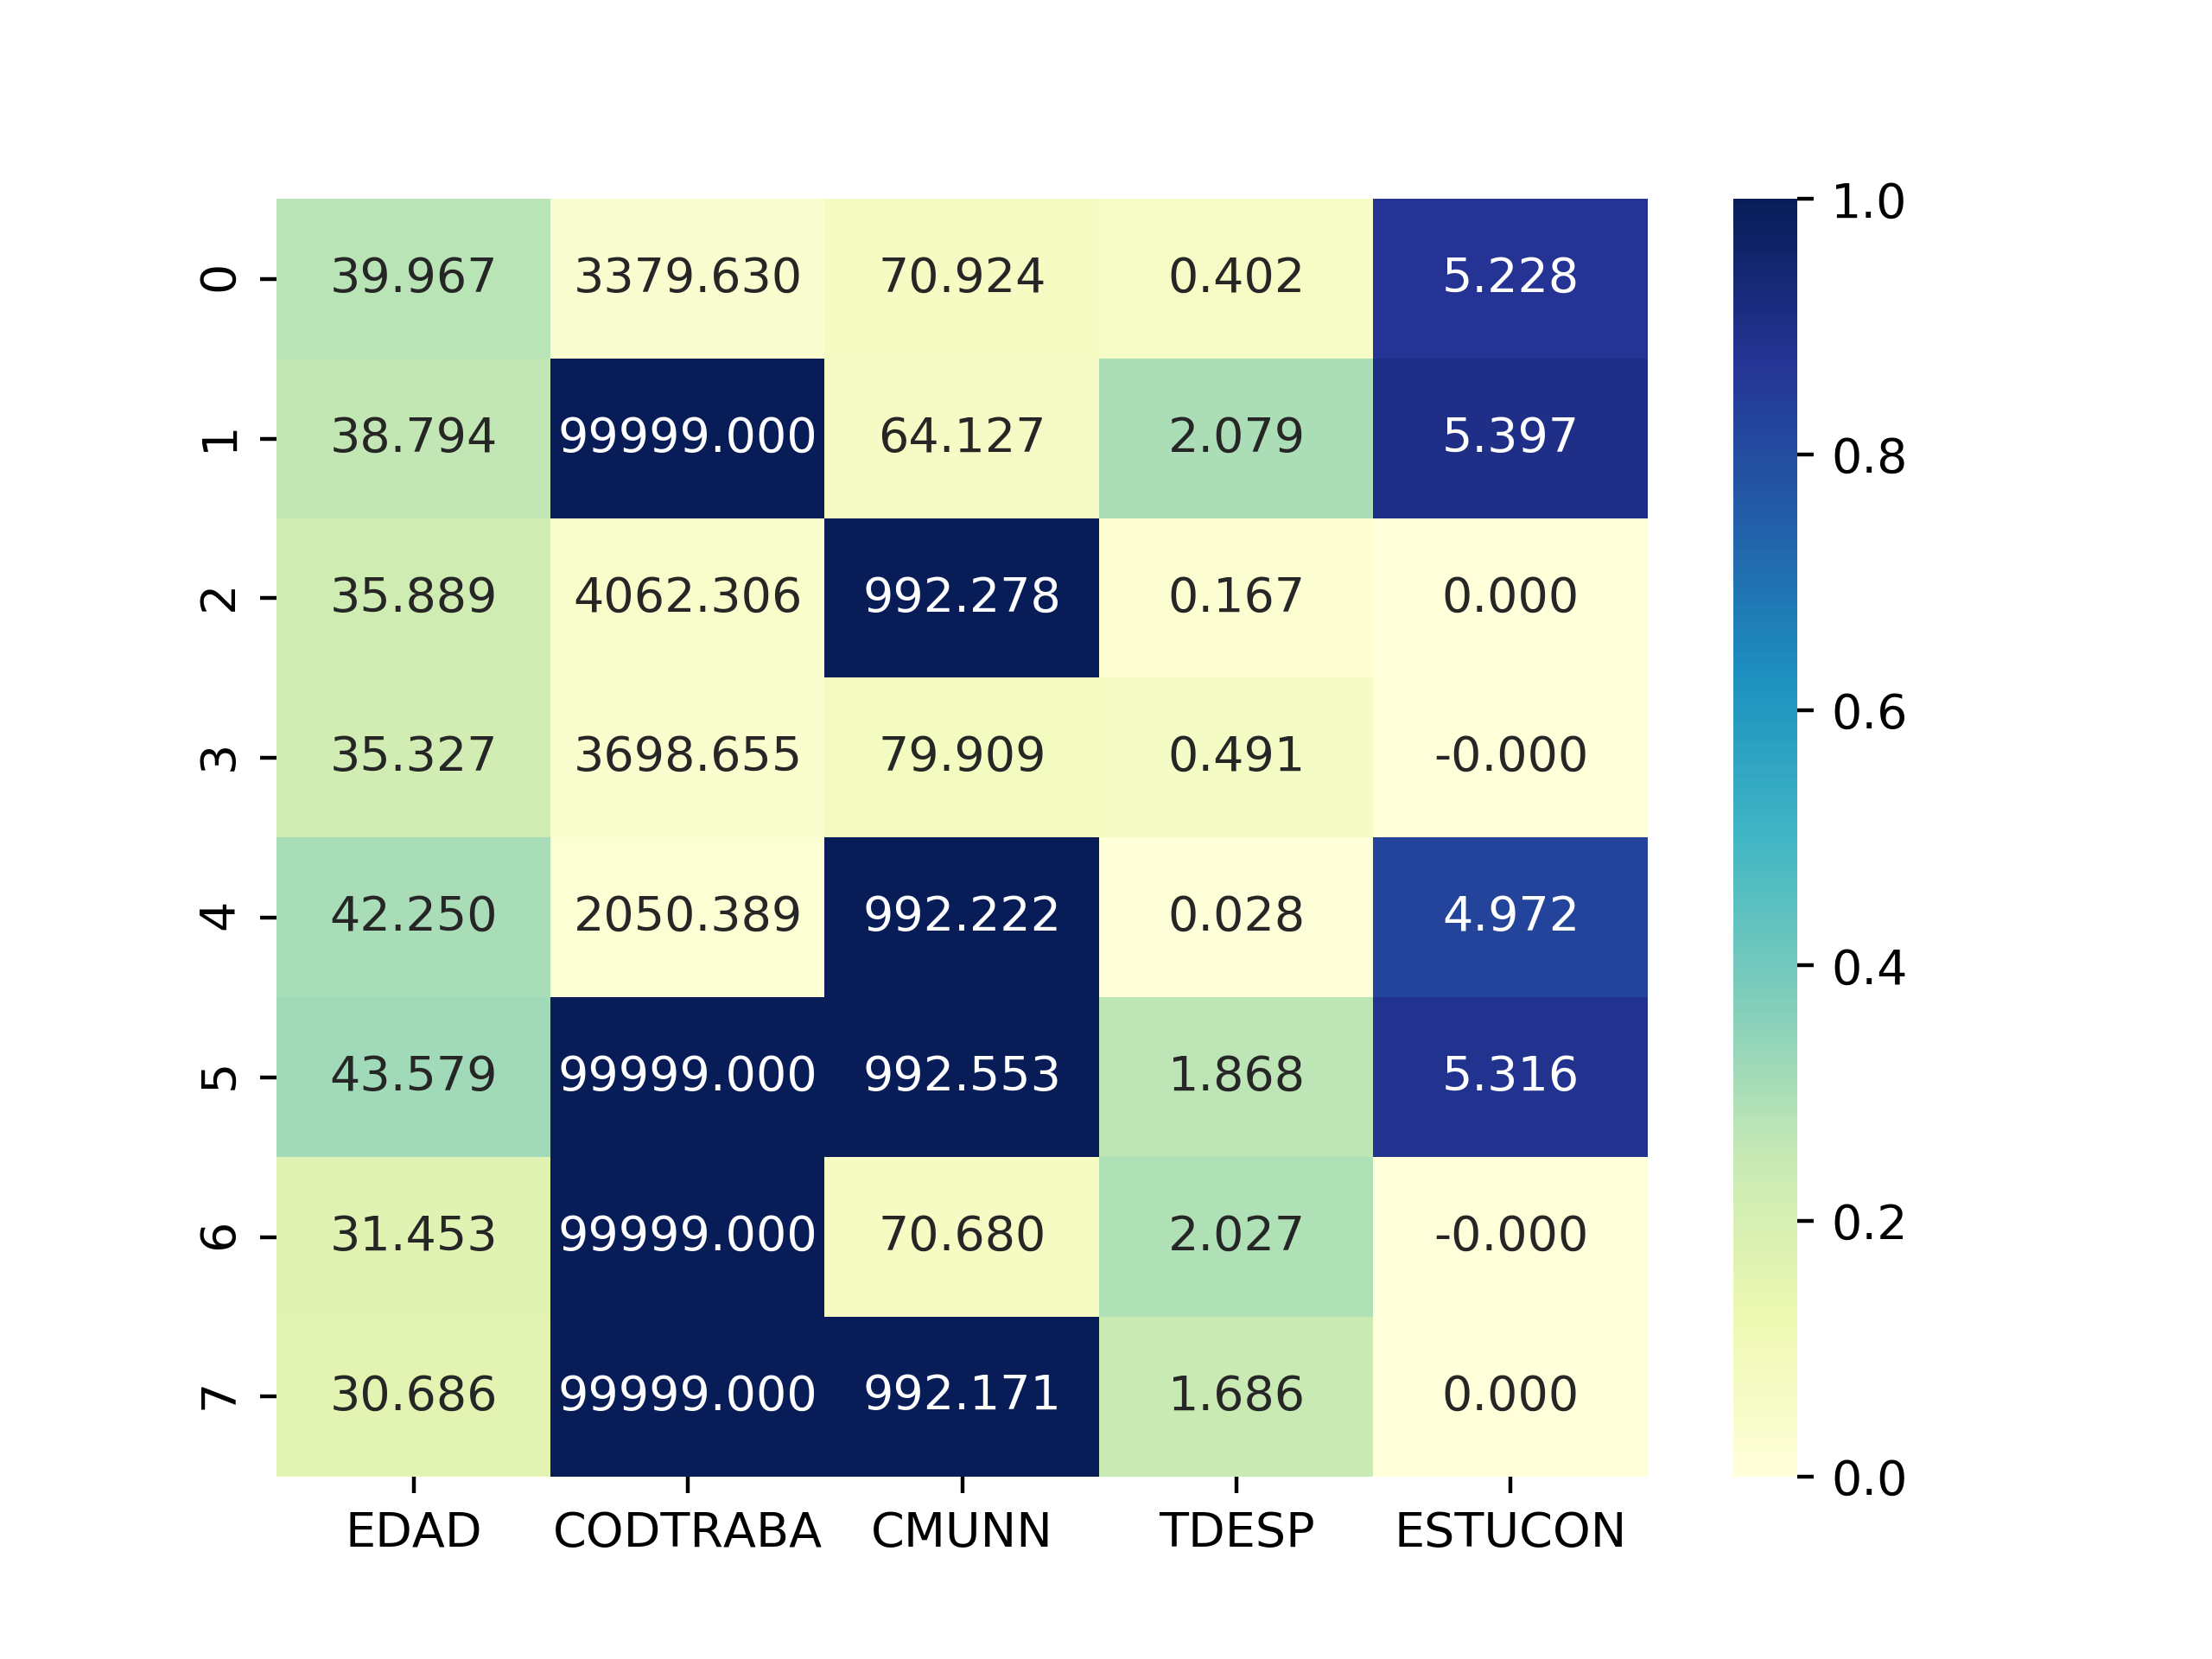
\includegraphics[scale=0.8]{heatmap-km-2.png}  %el parámetro scale permite agrandar o achicar la imagen. En el nombre de archivo puede especificar directorios
	\caption{Heatmap kMeans Caso 2} 
	\label{fig:hm-km-caso2}
\end{figure}

\begin{figure}[H] %con el [H] le obligamos a situar aquí la figura
	\centering
	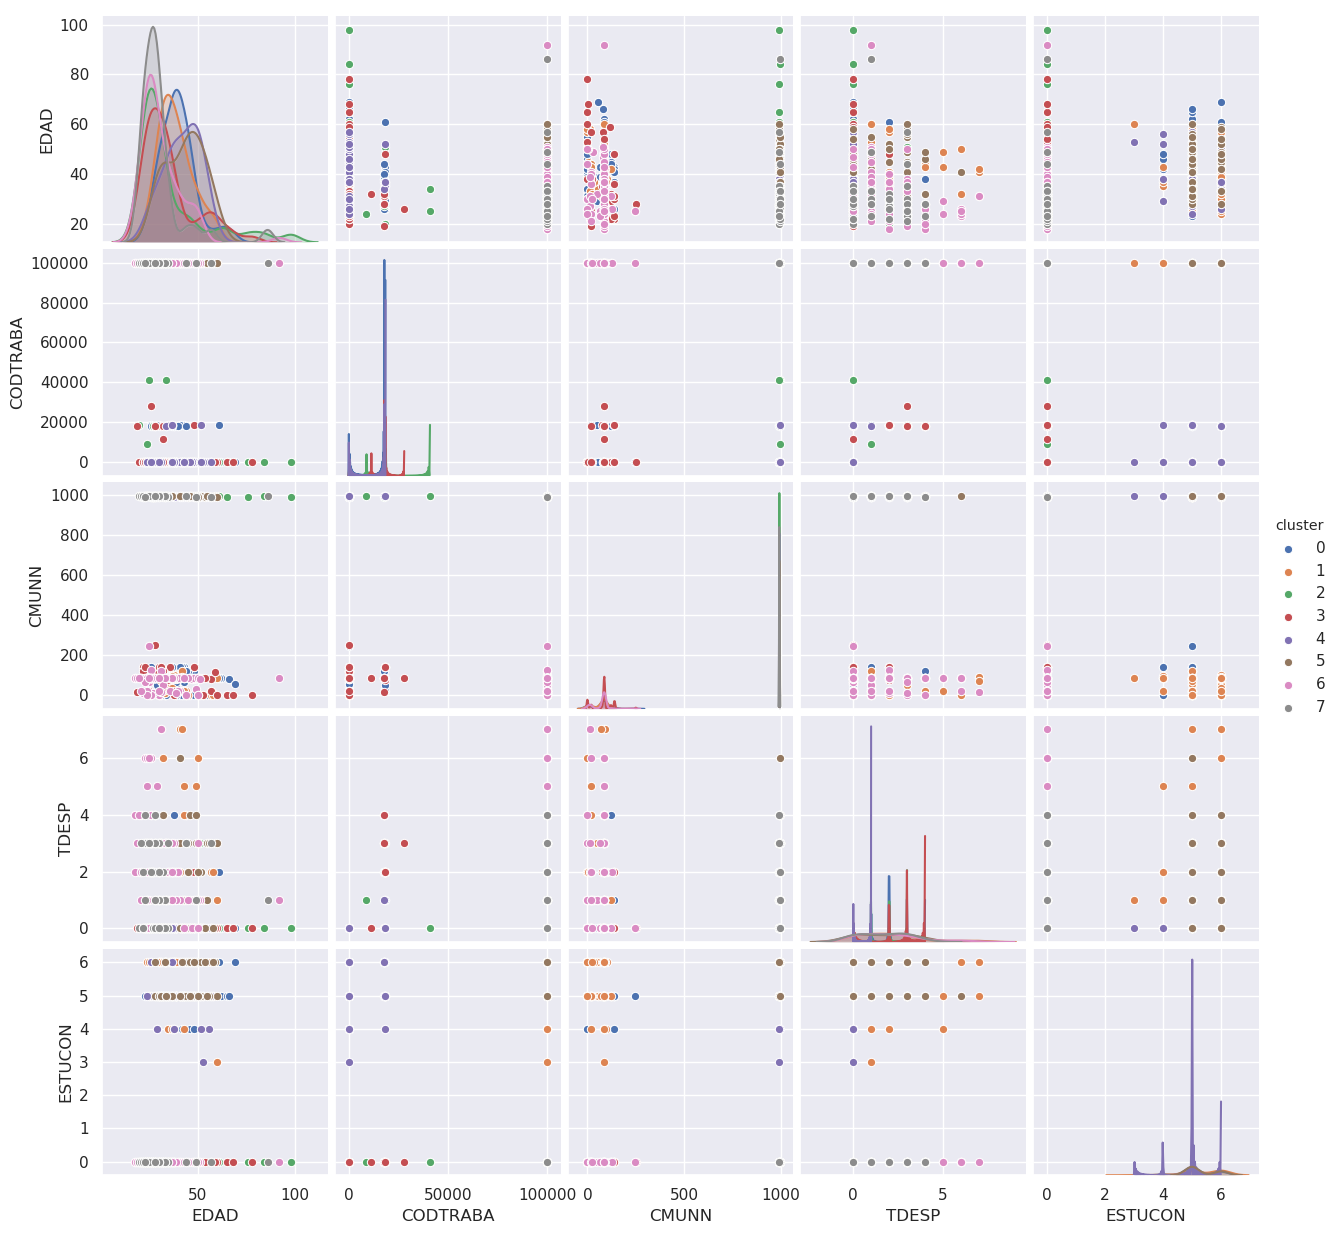
\includegraphics[scale=0.4]{kmeans-2.png}  %el parámetro scale permite agrandar o achicar la imagen. En el nombre de archivo puede especificar directorios
	\caption{Scatter kMeans Caso 2} 
	\label{fig:sc-km-caso2}
\end{figure}




\newpage

%----------------------------------------------------------------------------------------
%	Contenido adicional
%----------------------------------------------------------------------------------------

\section{Contenido adicional}




\newpage
\section{Bibliografía}

%------------------------------------------------

\bibliography{citas} %archivo citas.bib que contiene las entradas 
\bibliographystyle{plain} % hay varias formas de citar

\end{document}
